%------------------------------------------------------------------
\chapter{Galáxias com linhas de absorção.}\label{app:abs}
%------------------------------------------------------------------
%\begin{comment}
\begin{figure}[H]
    \begin{center}
        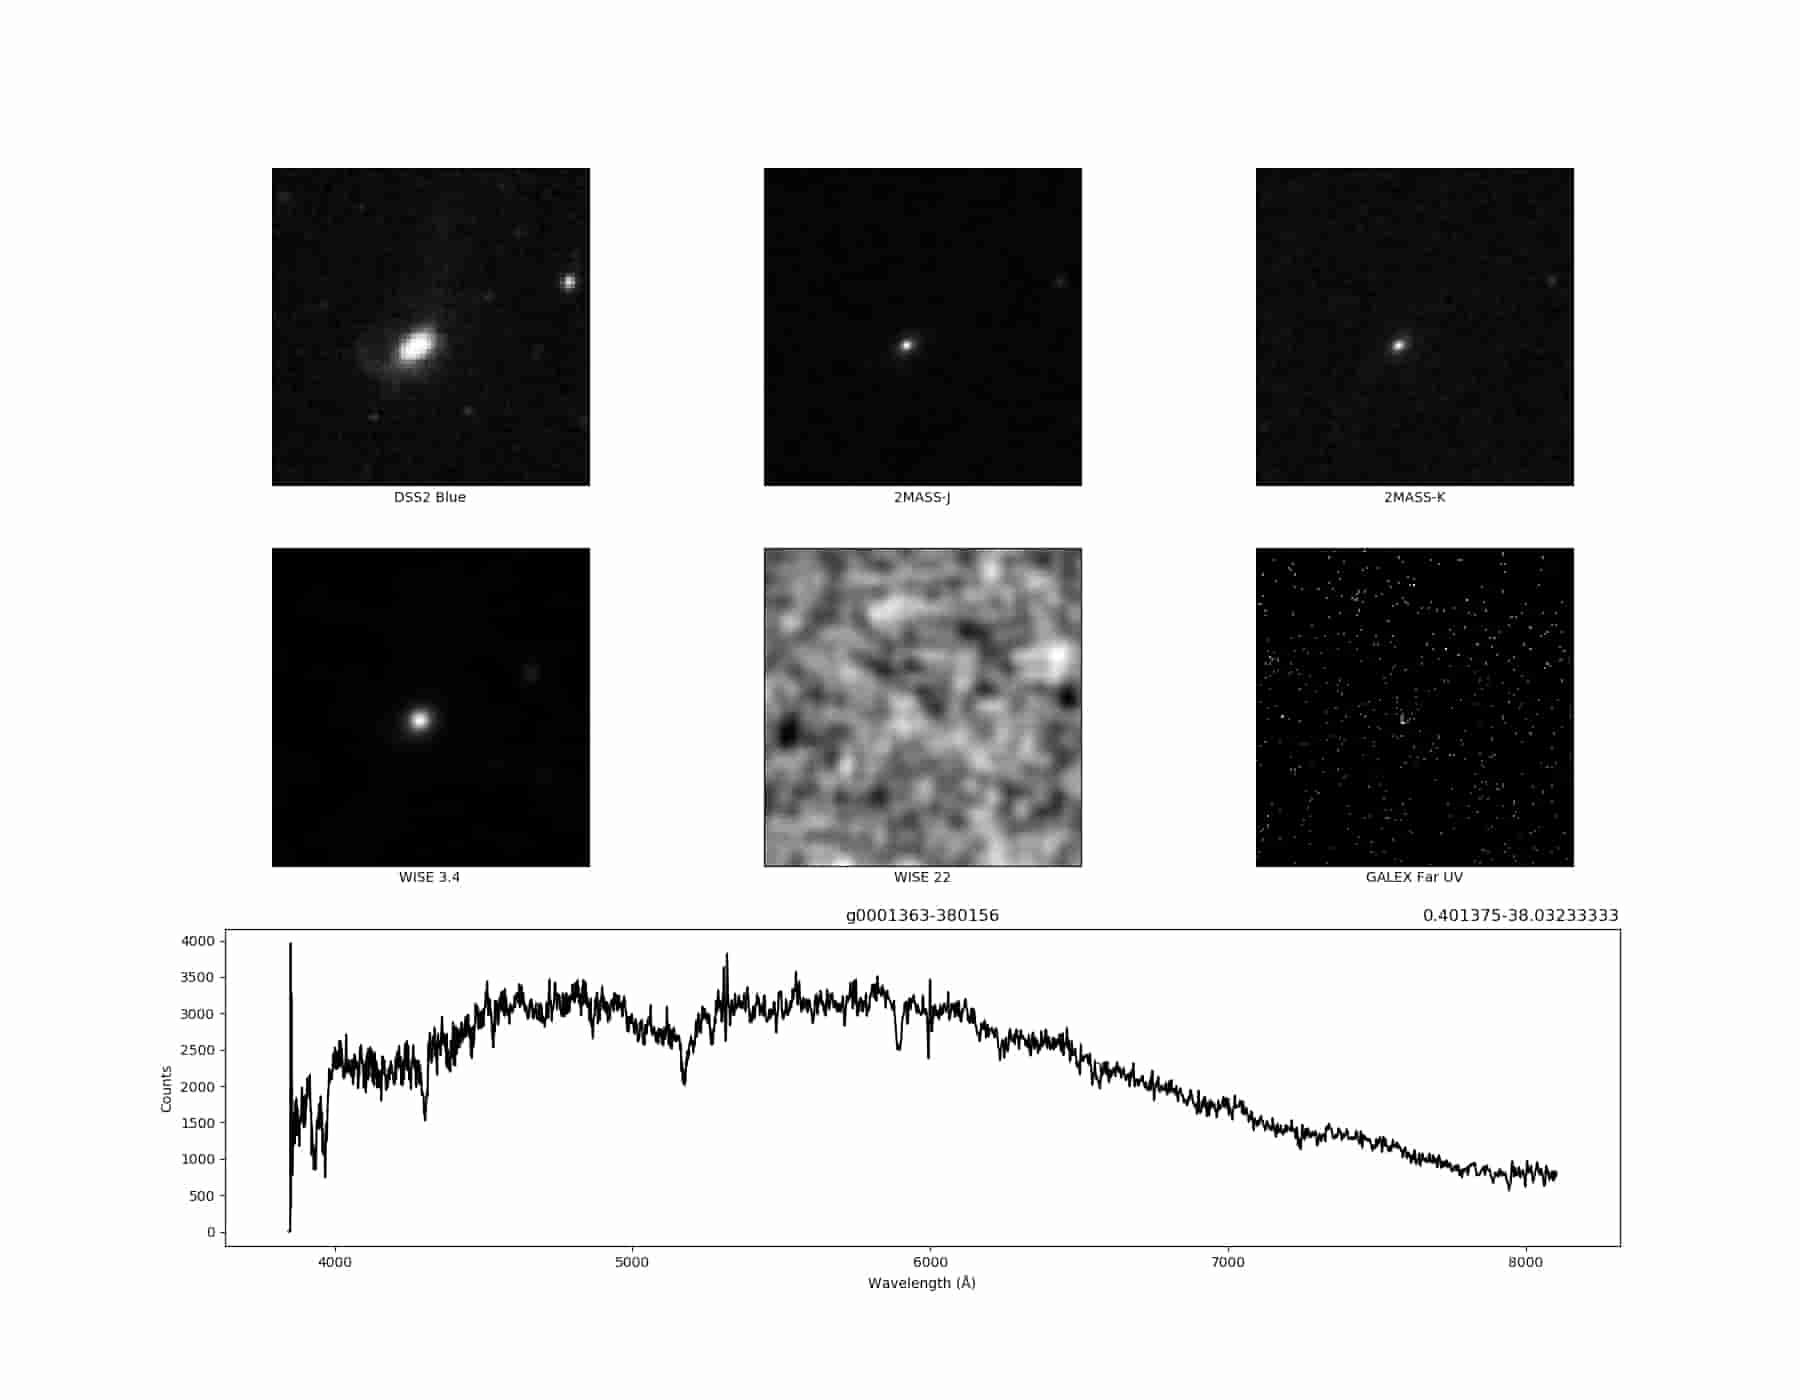
\includegraphics[scale = 0.10]{figuras/1.jpg}
        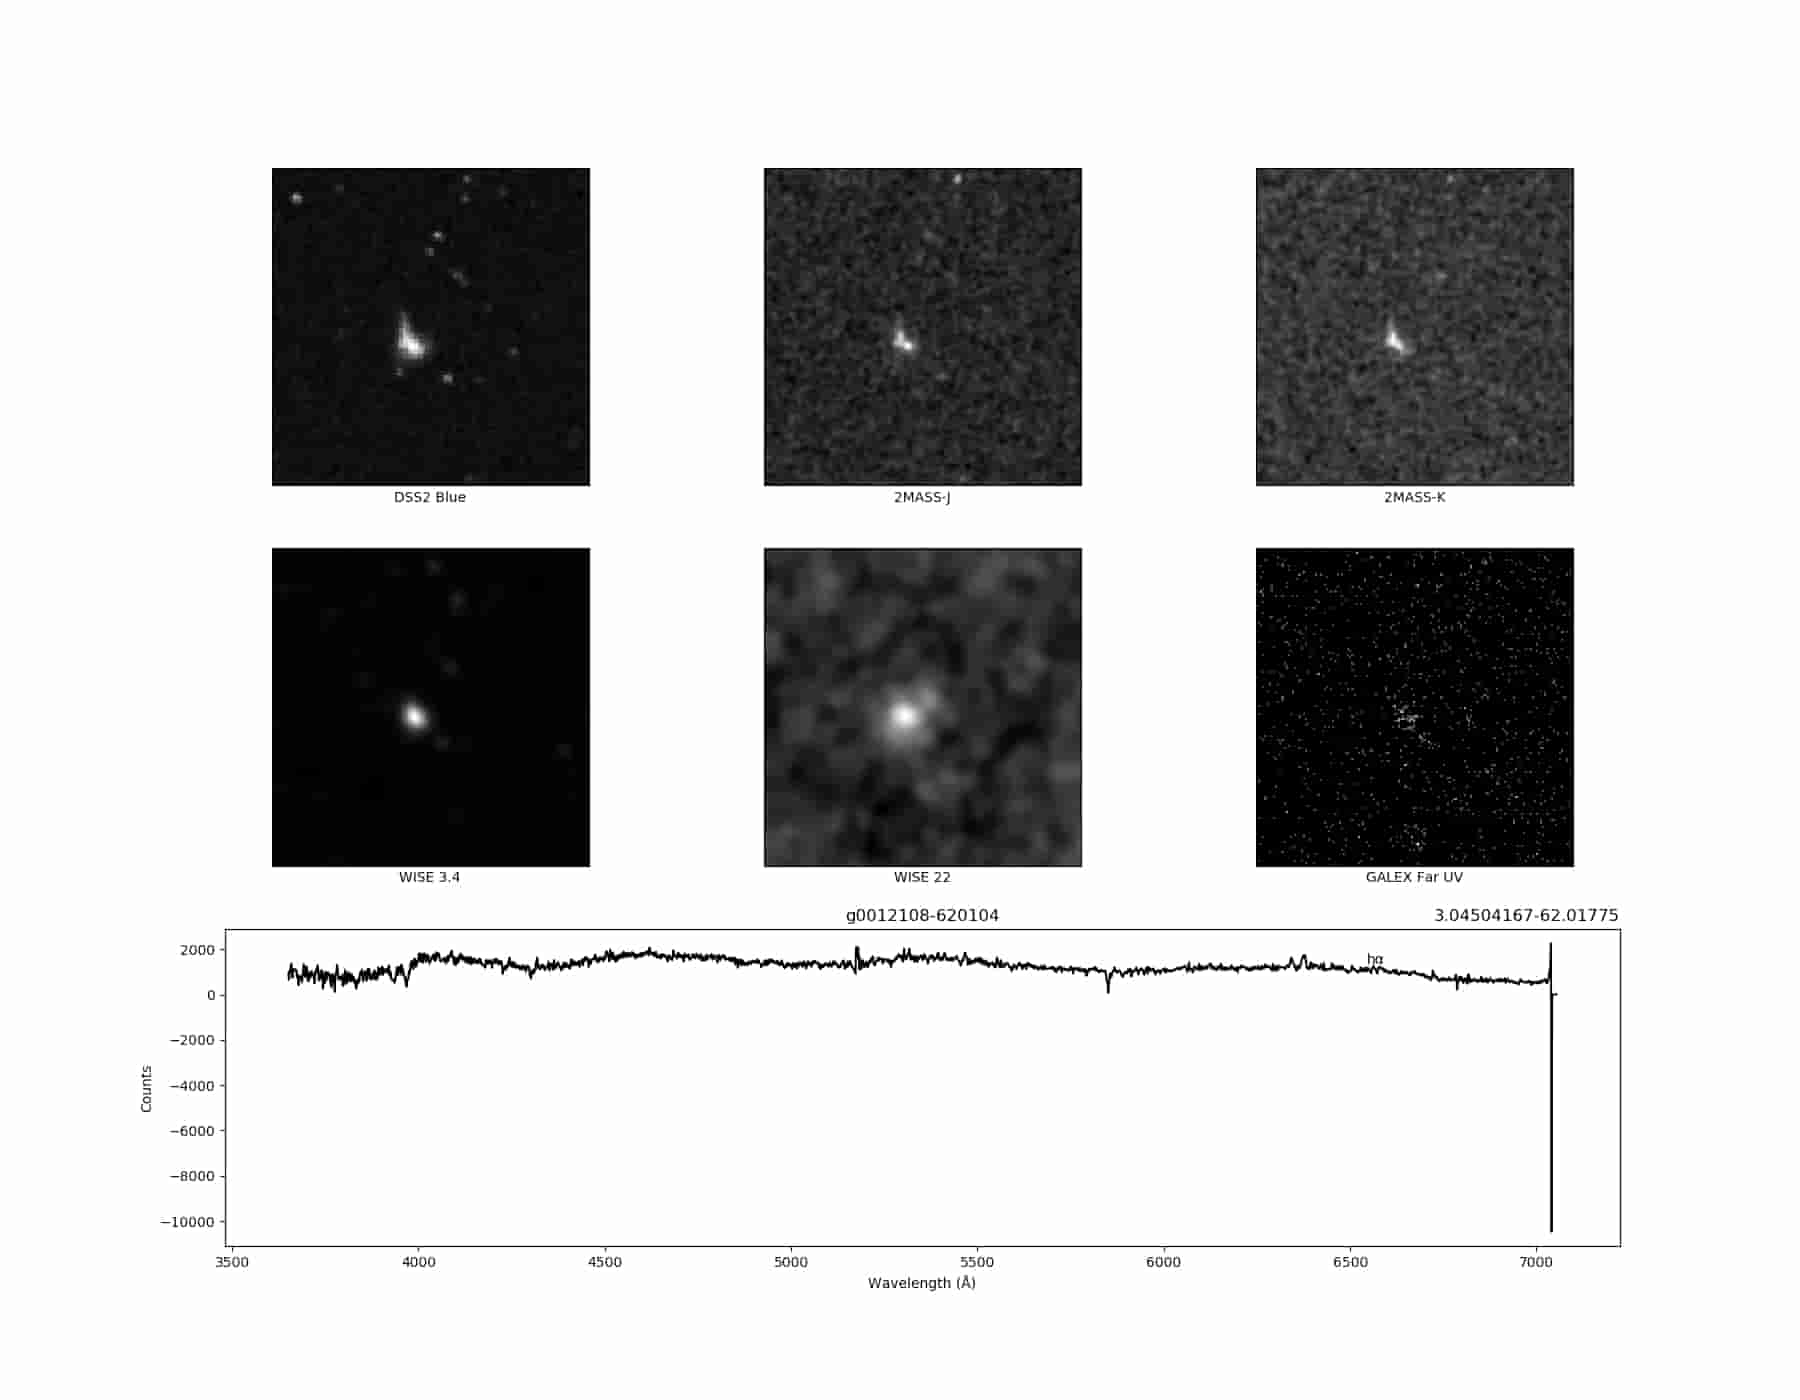
\includegraphics[scale = 0.10]{figuras/2.jpg}
        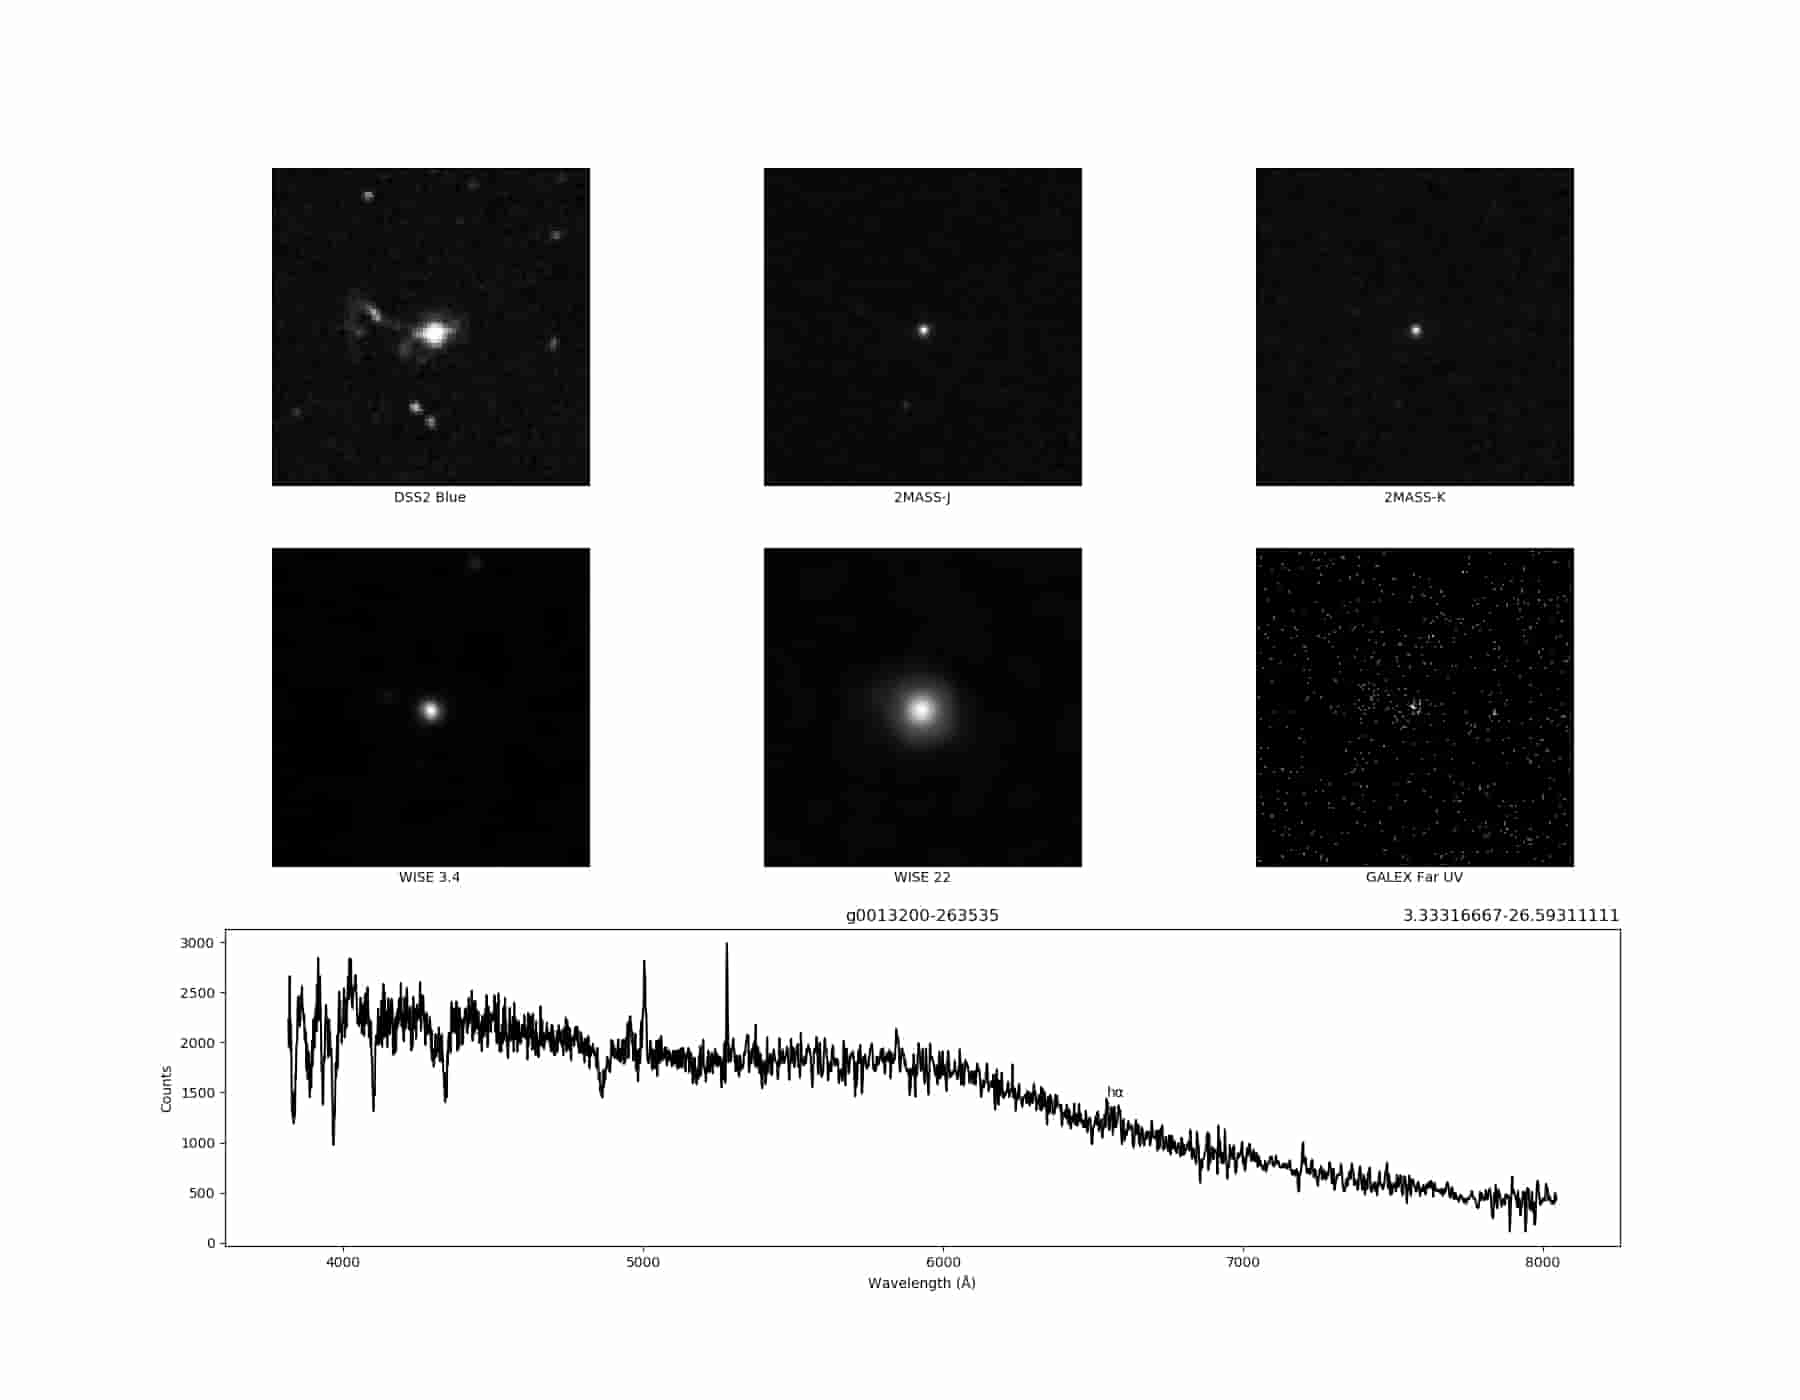
\includegraphics[scale = 0.10]{figuras/3.jpg}
        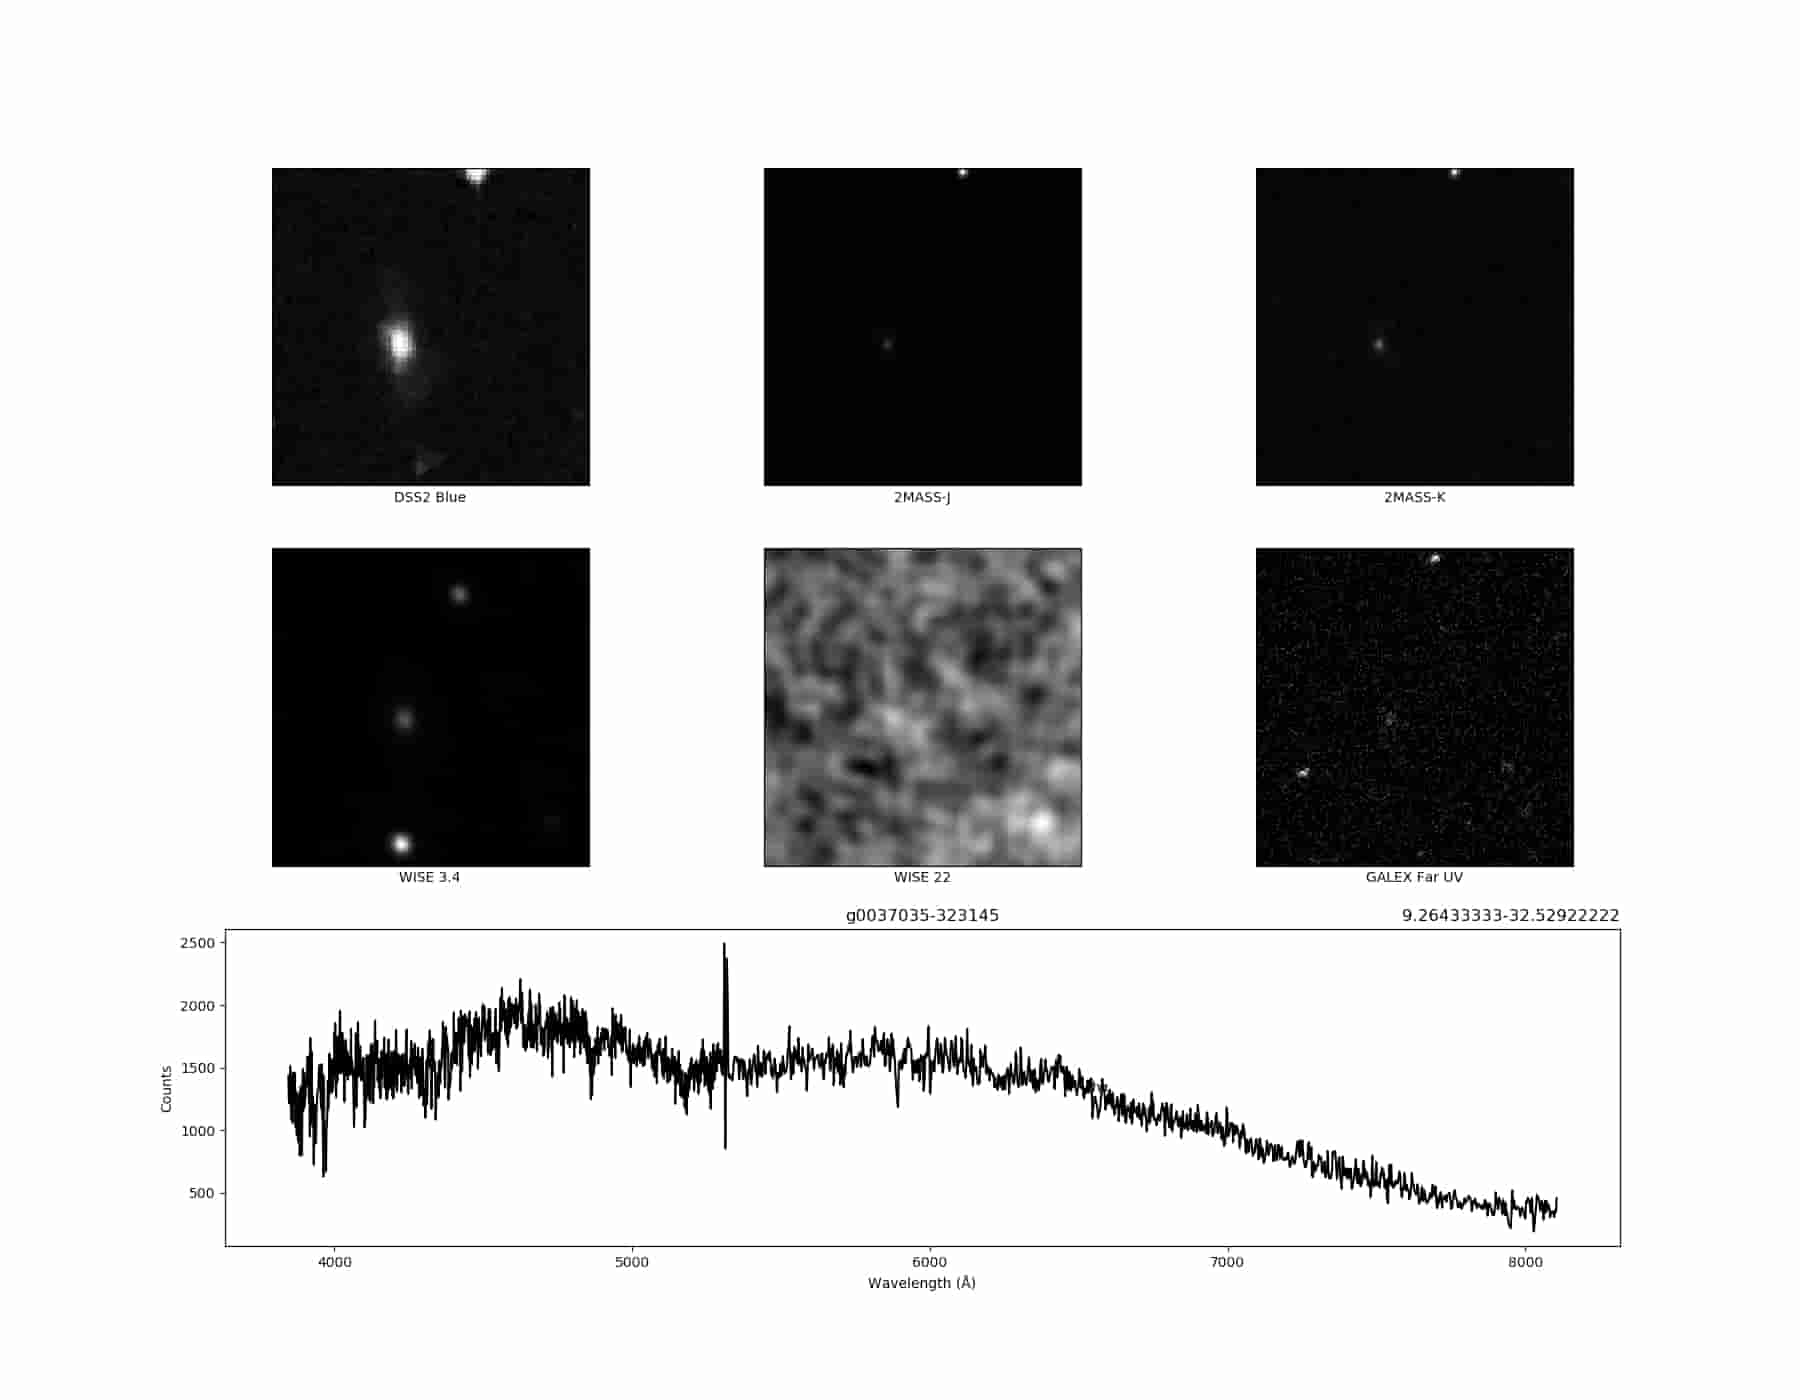
\includegraphics[scale = 0.10]{figuras/4.jpg}
        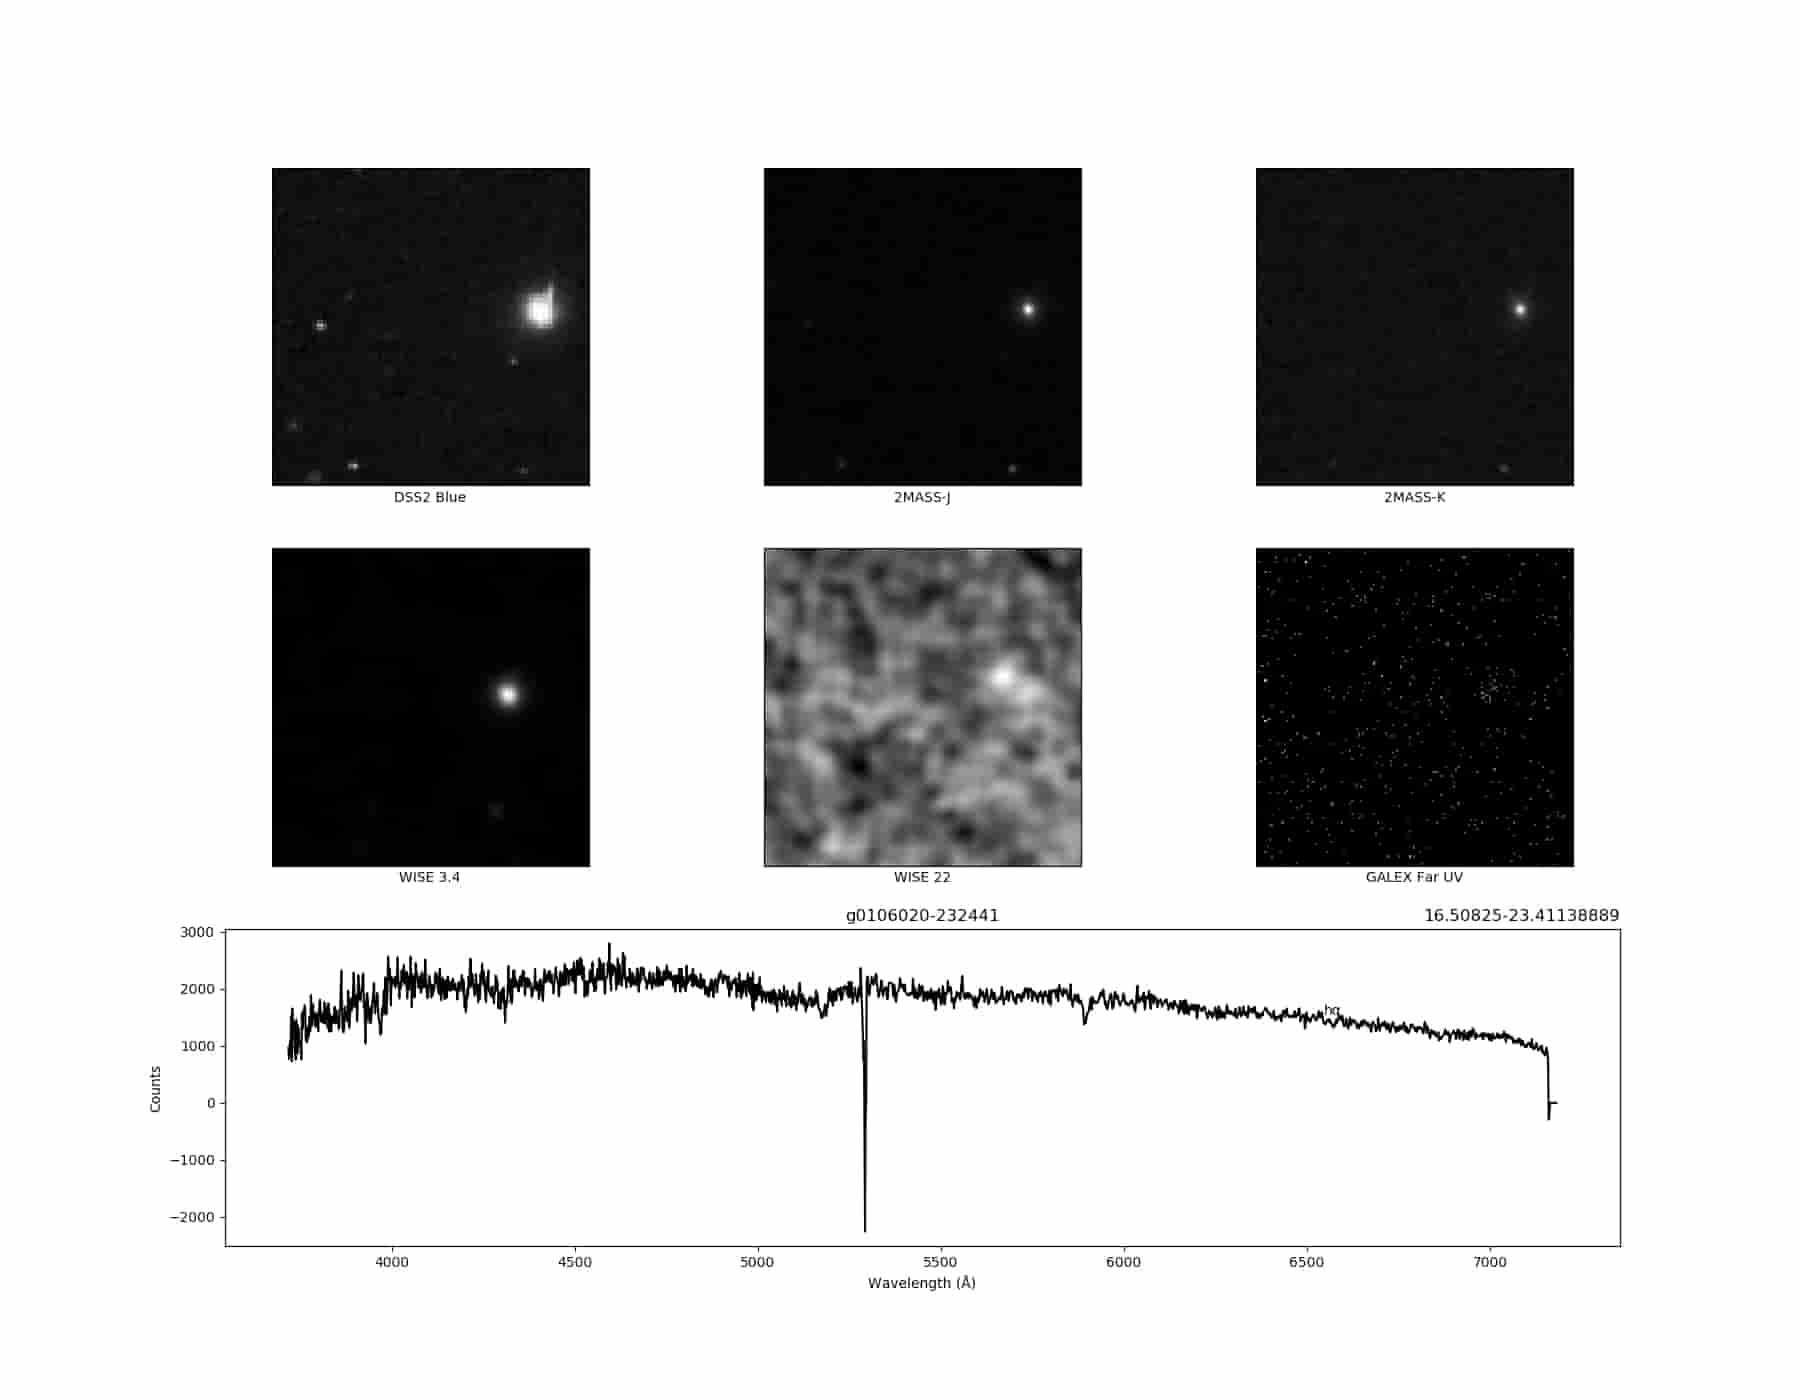
\includegraphics[scale = 0.10]{figuras/5.jpg}
        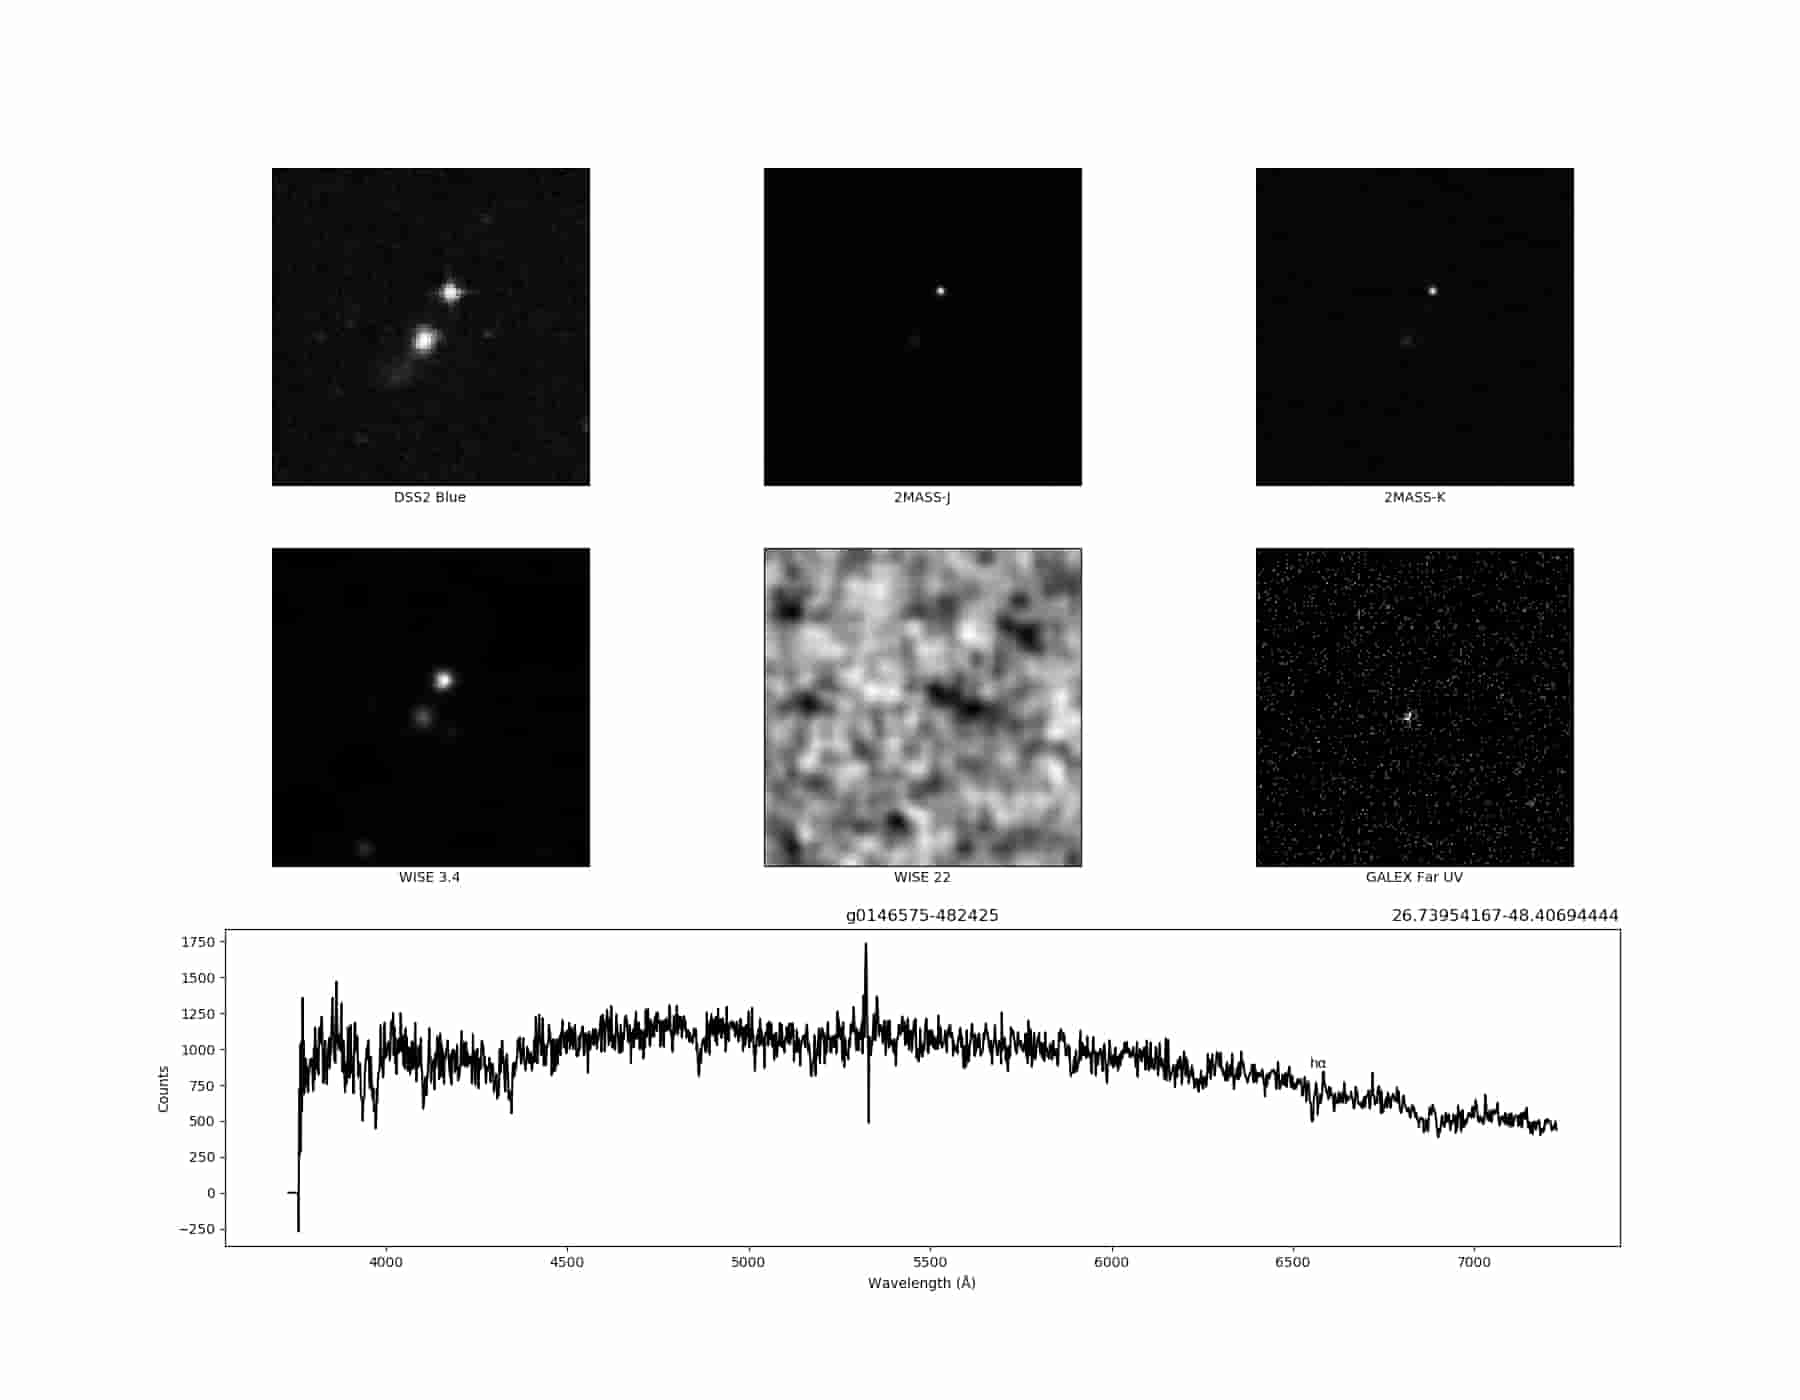
\includegraphics[scale = 0.10]{figuras/6.jpg}
        %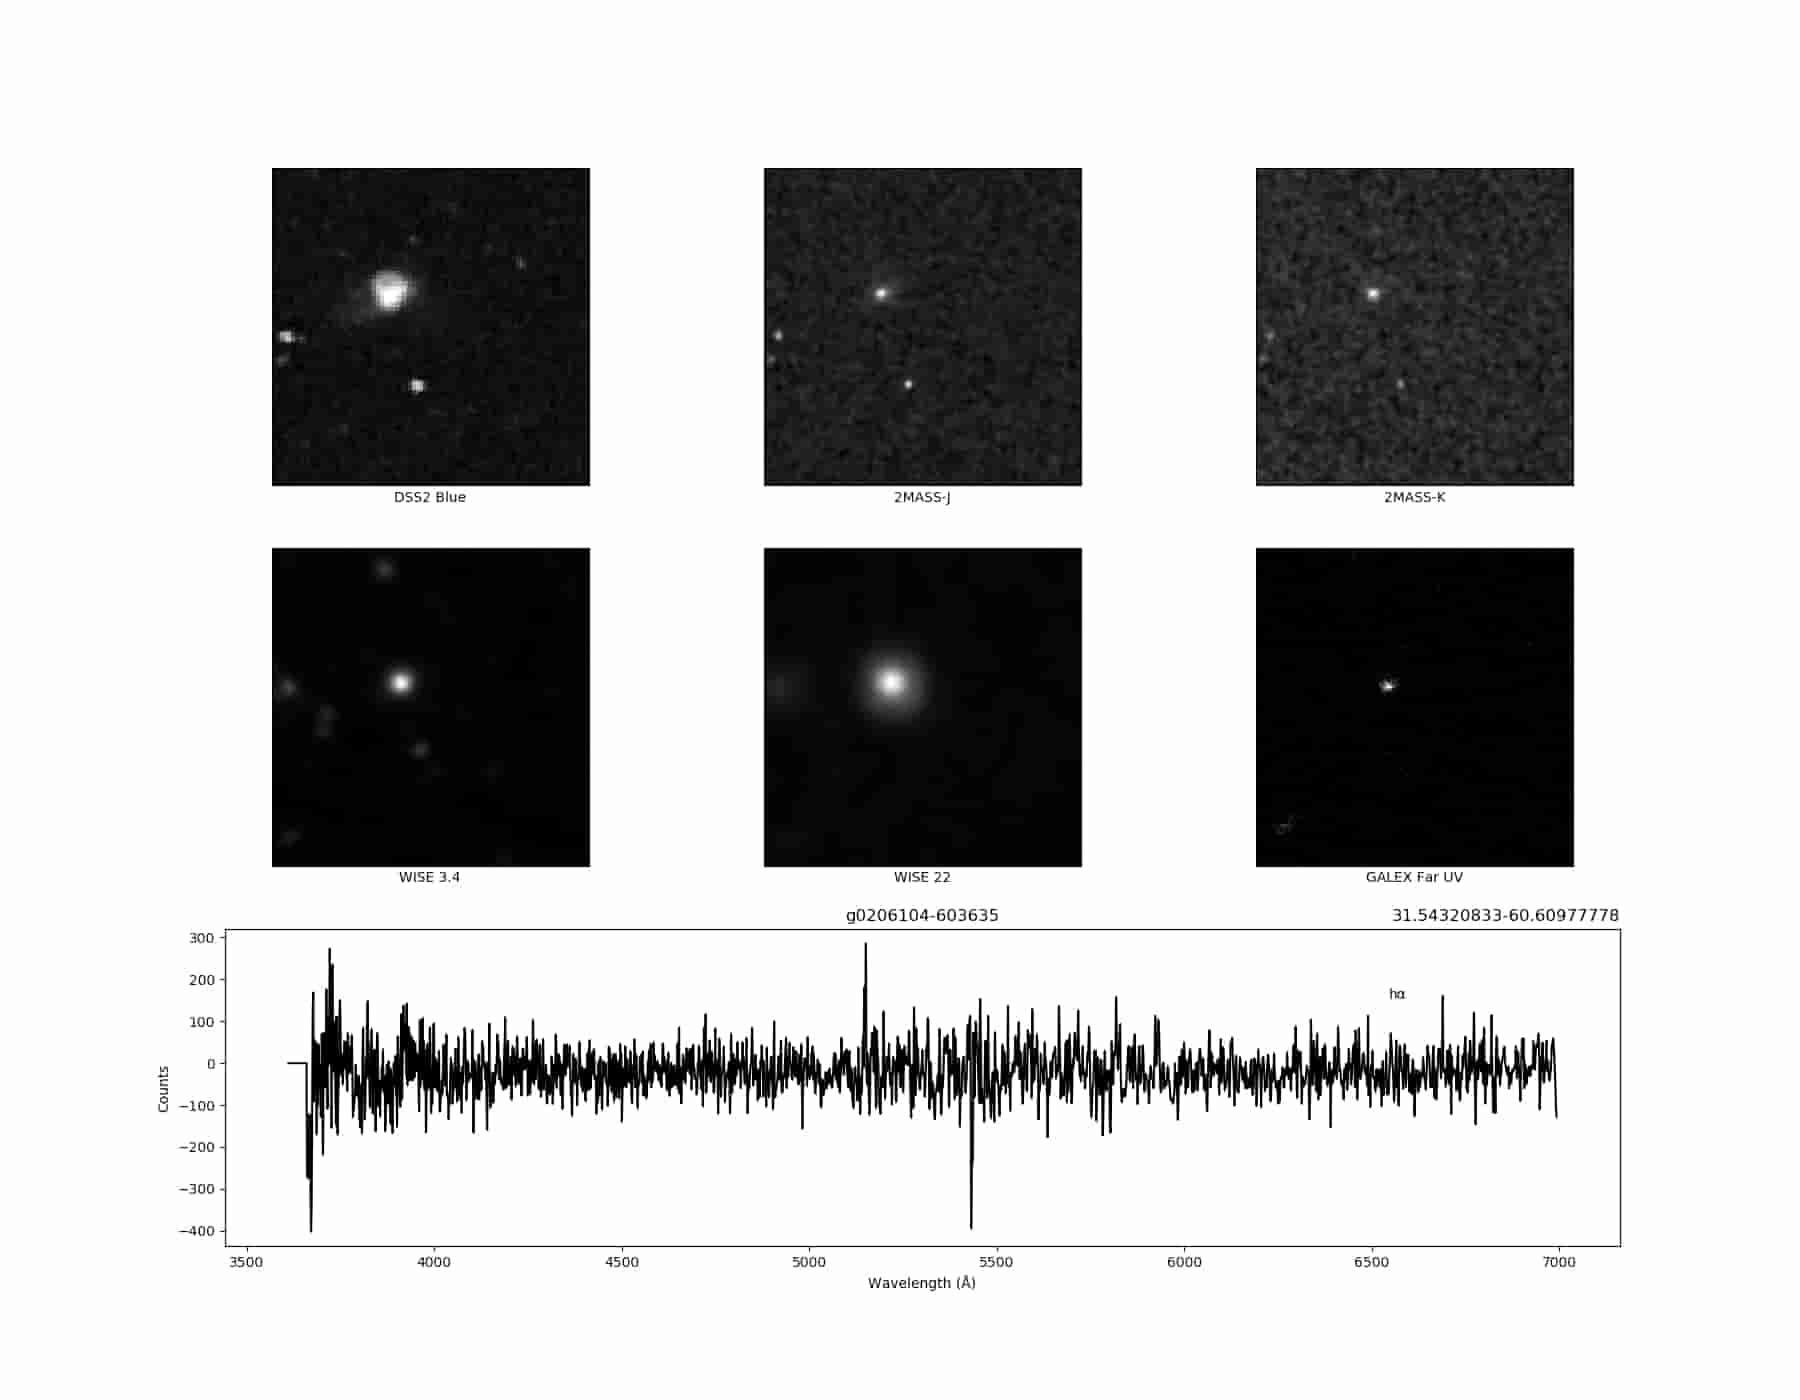
\includegraphics[scale = 0.08]{figuras/7.jpg}
        %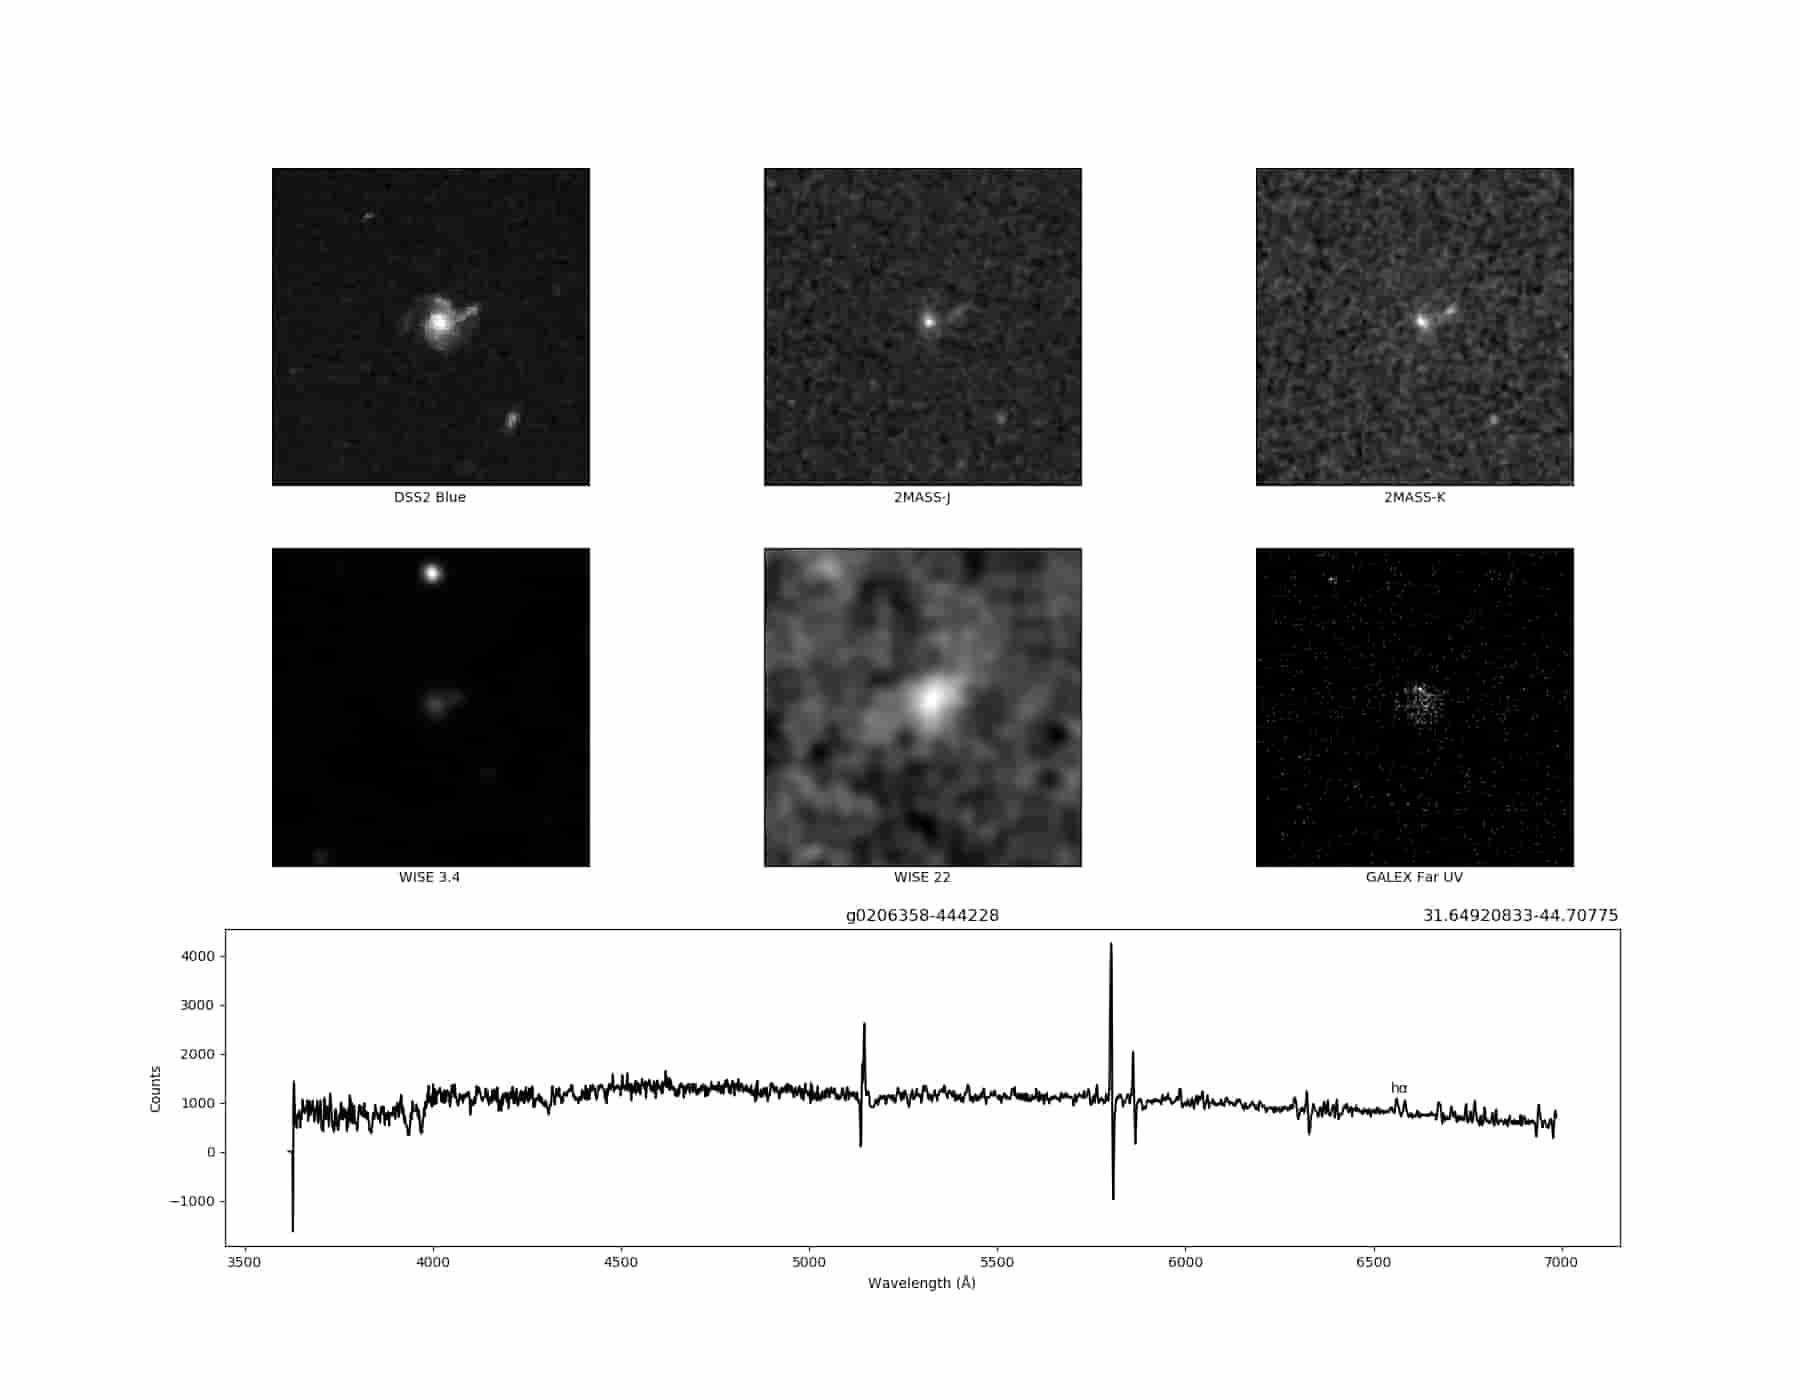
\includegraphics[scale = 0.08]{figuras/8.jpg}
        \label{fig:my_label}
    \end{center}
\end{figure}
%\end{comment}

\chapter{Galáxias com linhas de emissão.}
\begin{figure}[H]
    \begin{center}
        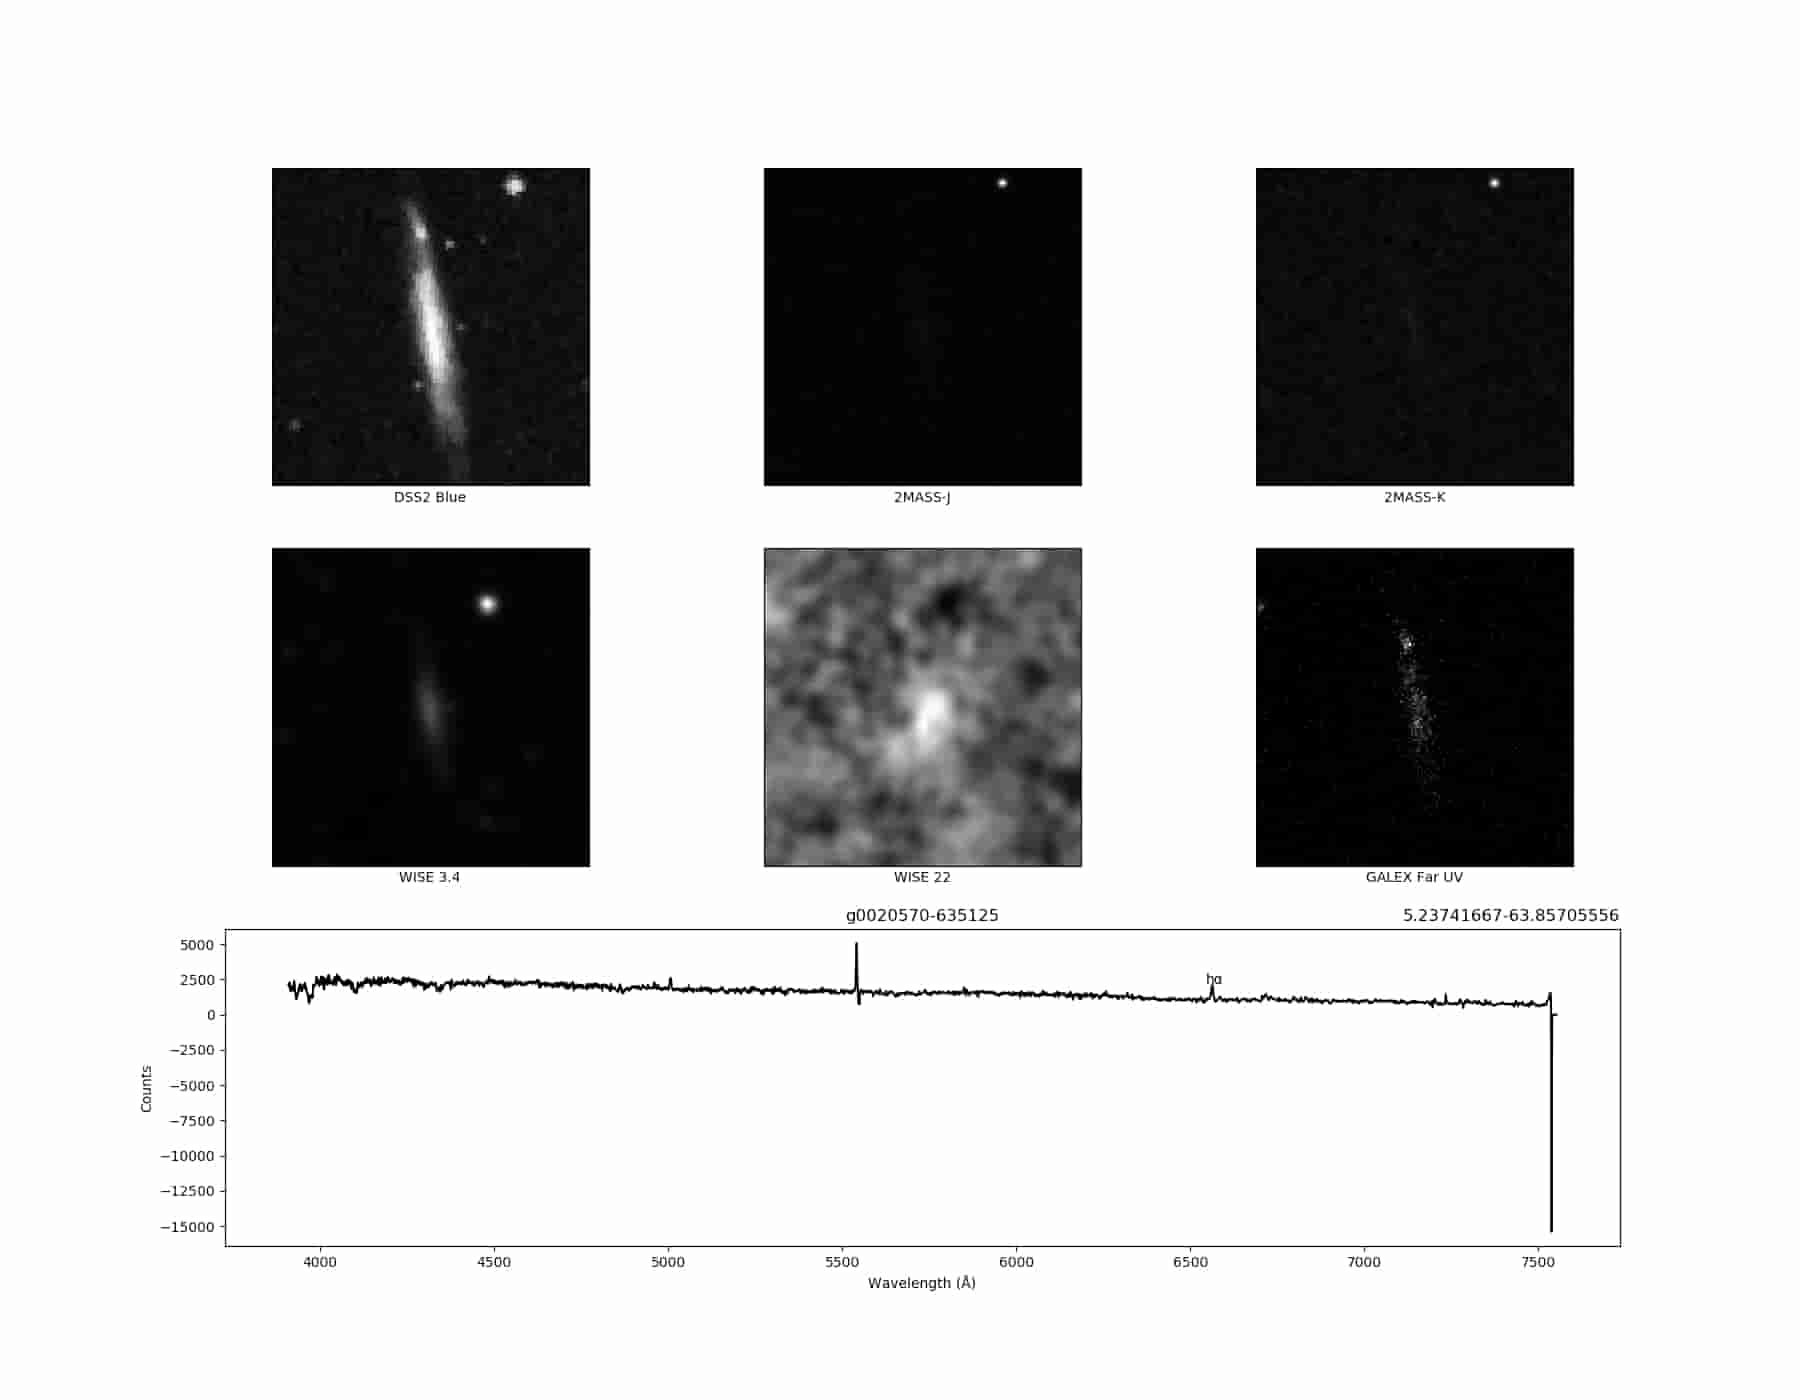
\includegraphics[scale = 0.10]{figuras/a1.jpg}
        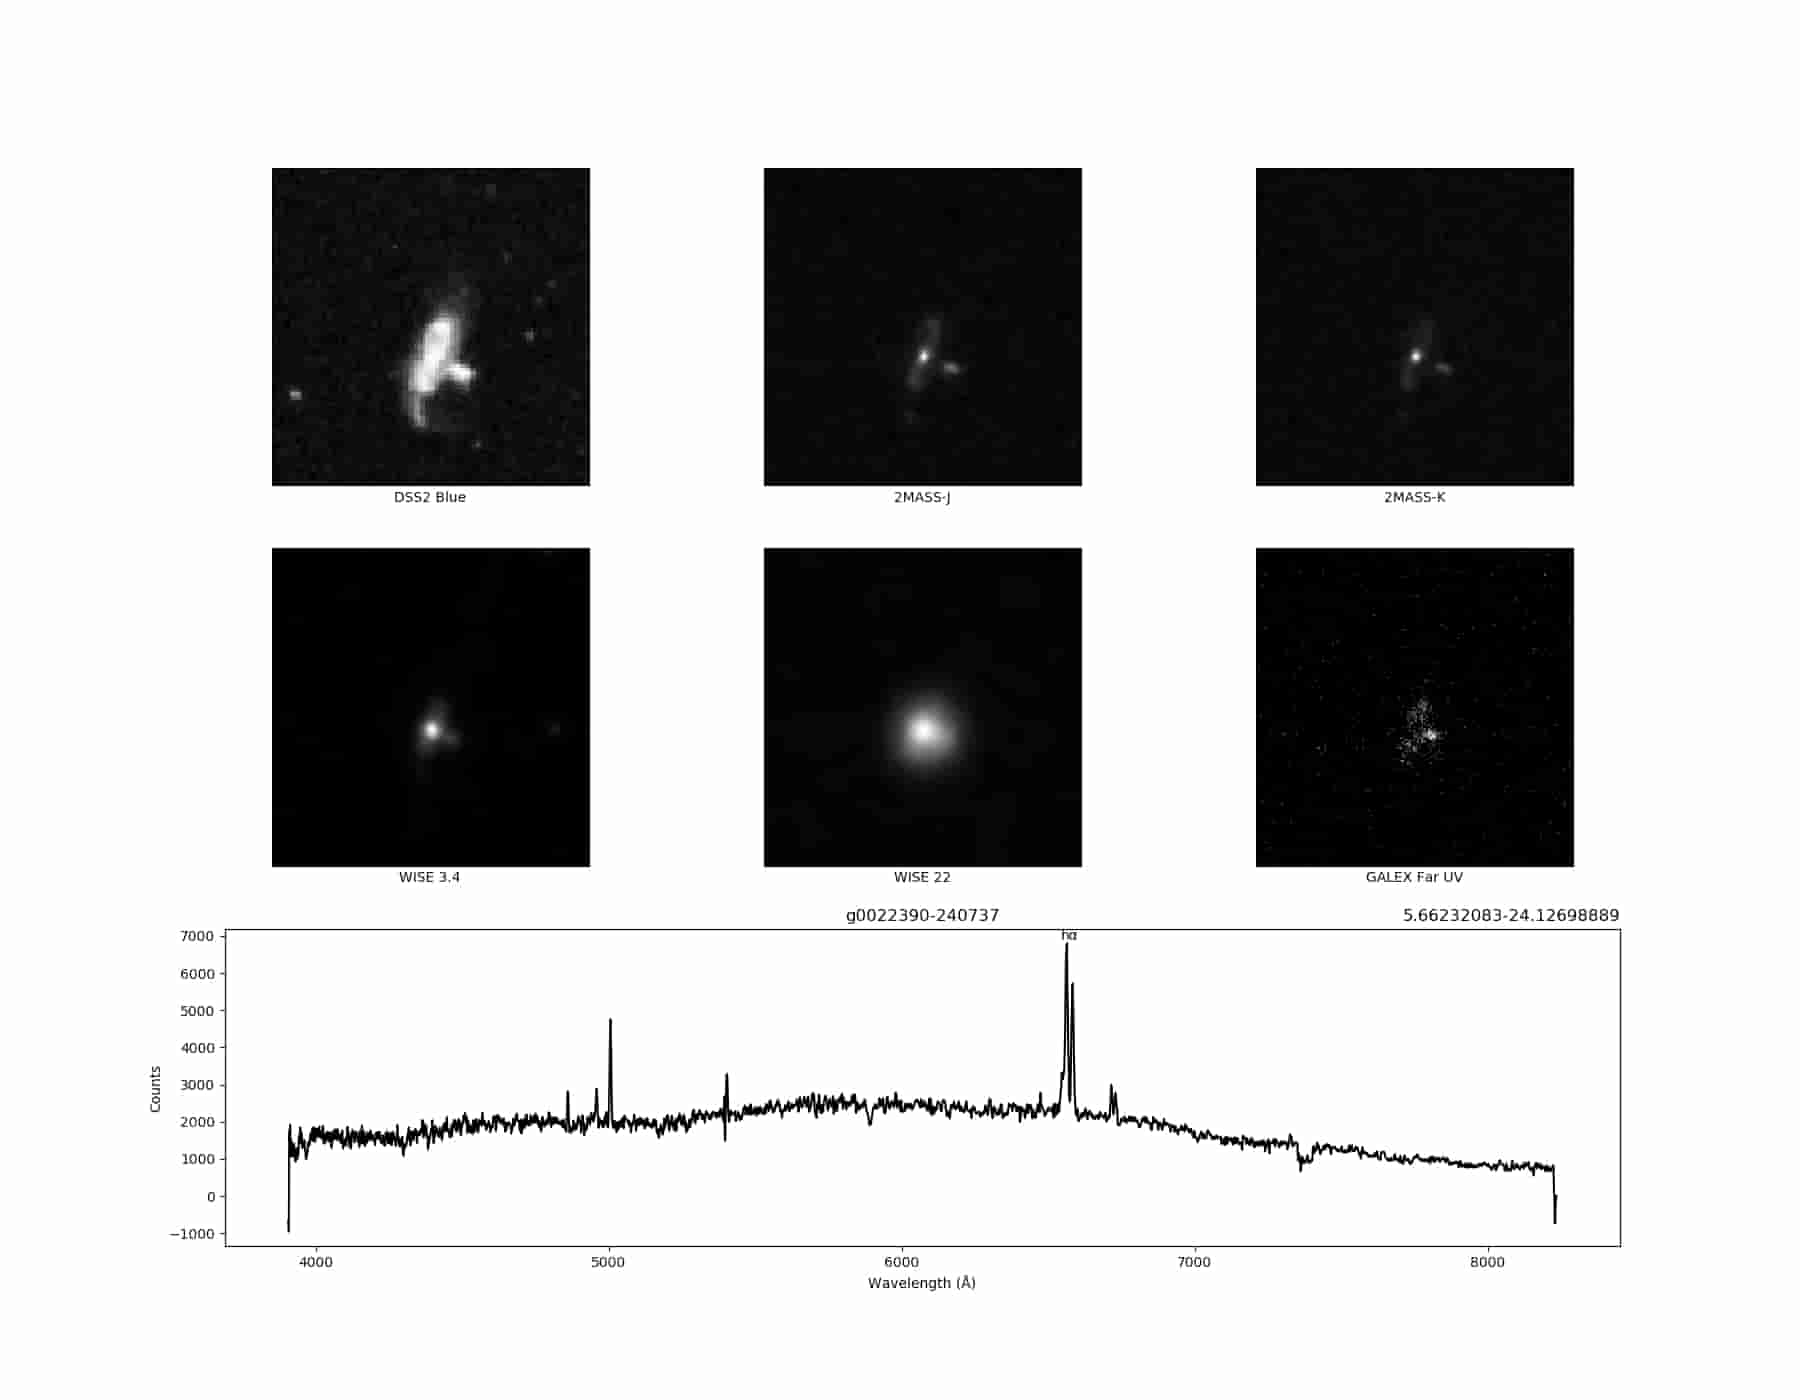
\includegraphics[scale = 0.10]{figuras/a2.jpg}
        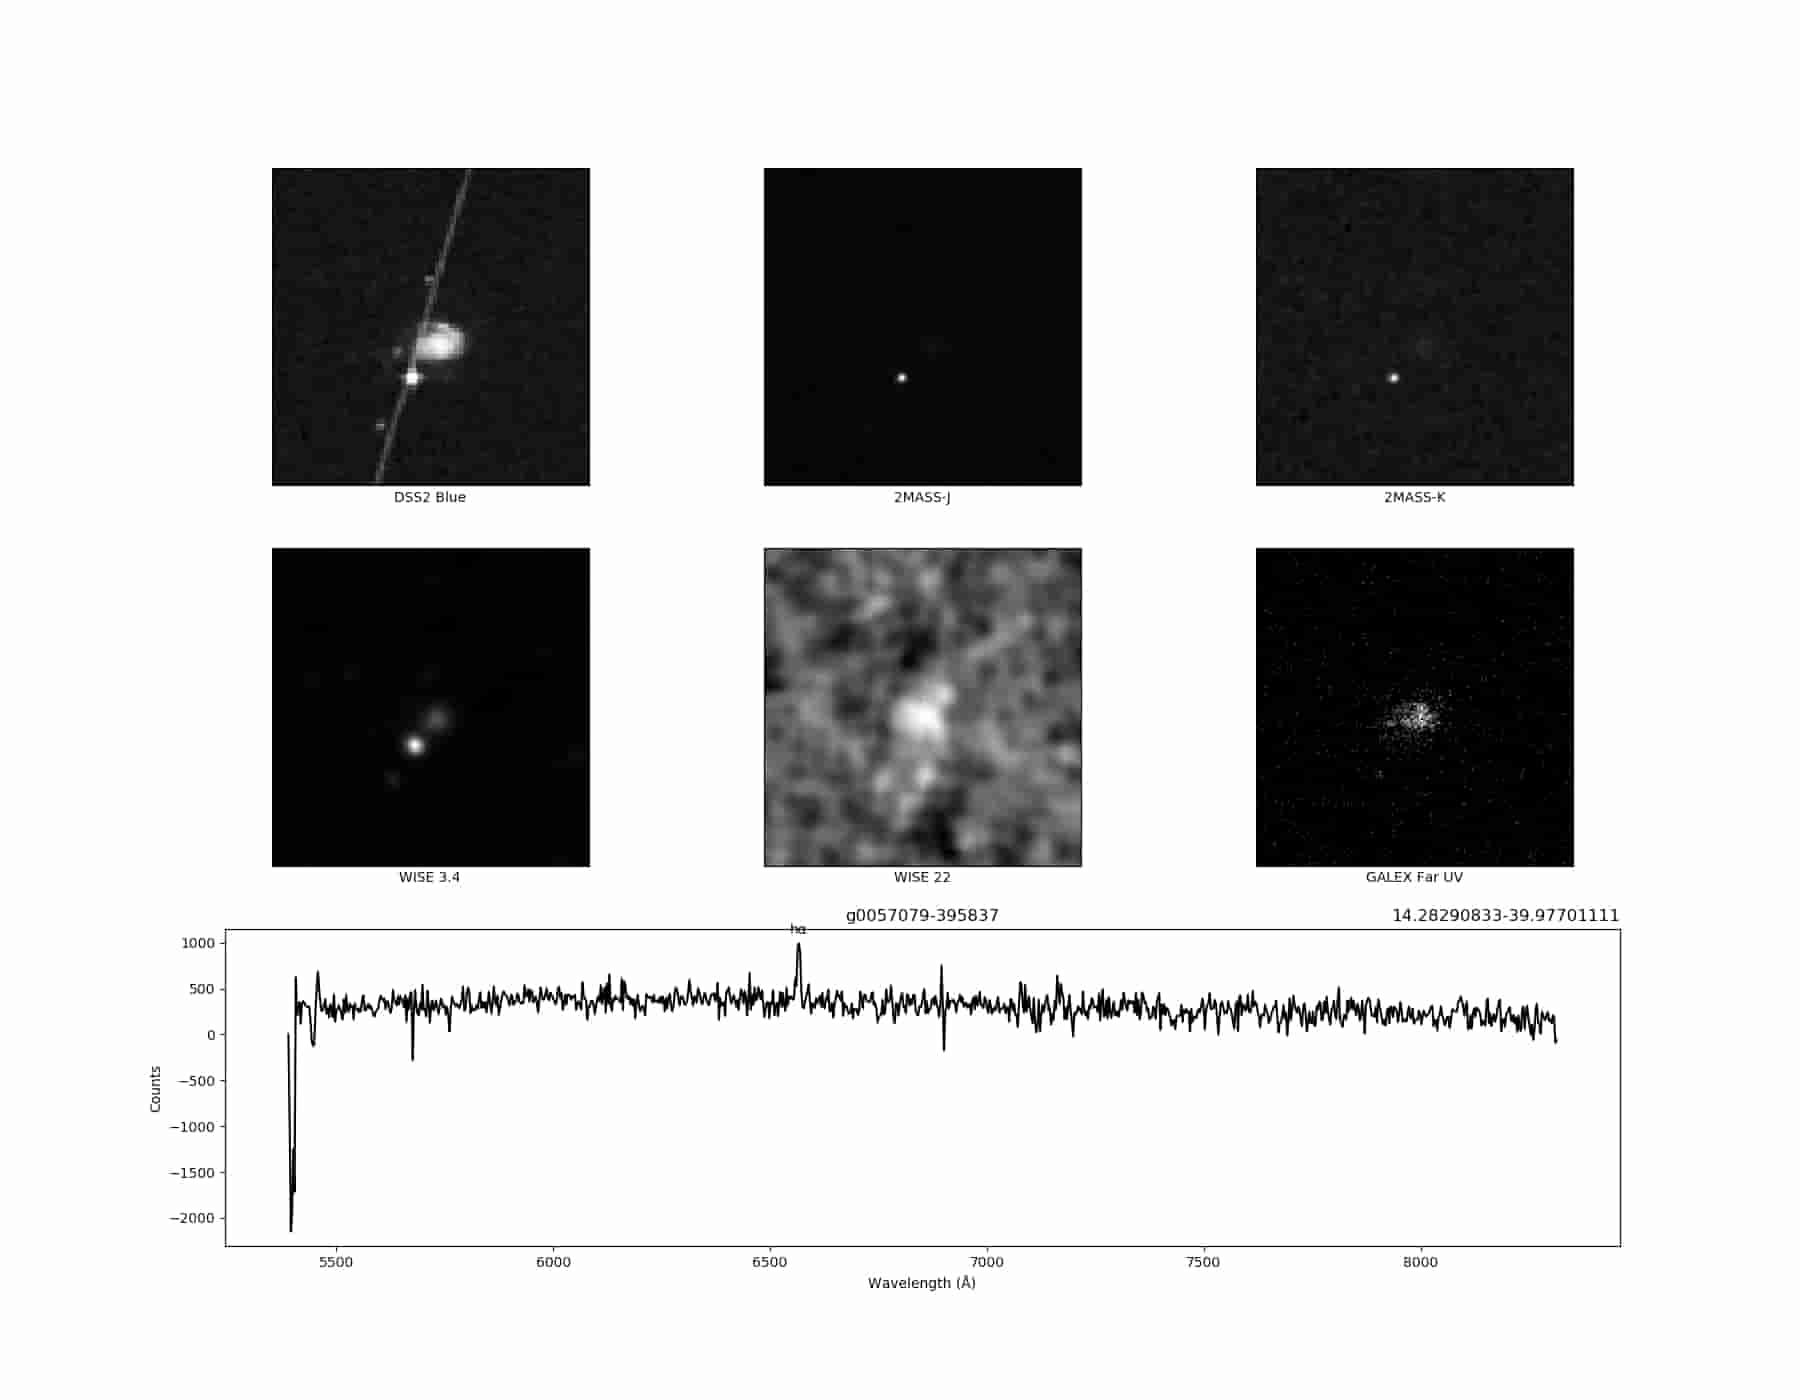
\includegraphics[scale = 0.10]{figuras/a3.jpg}
        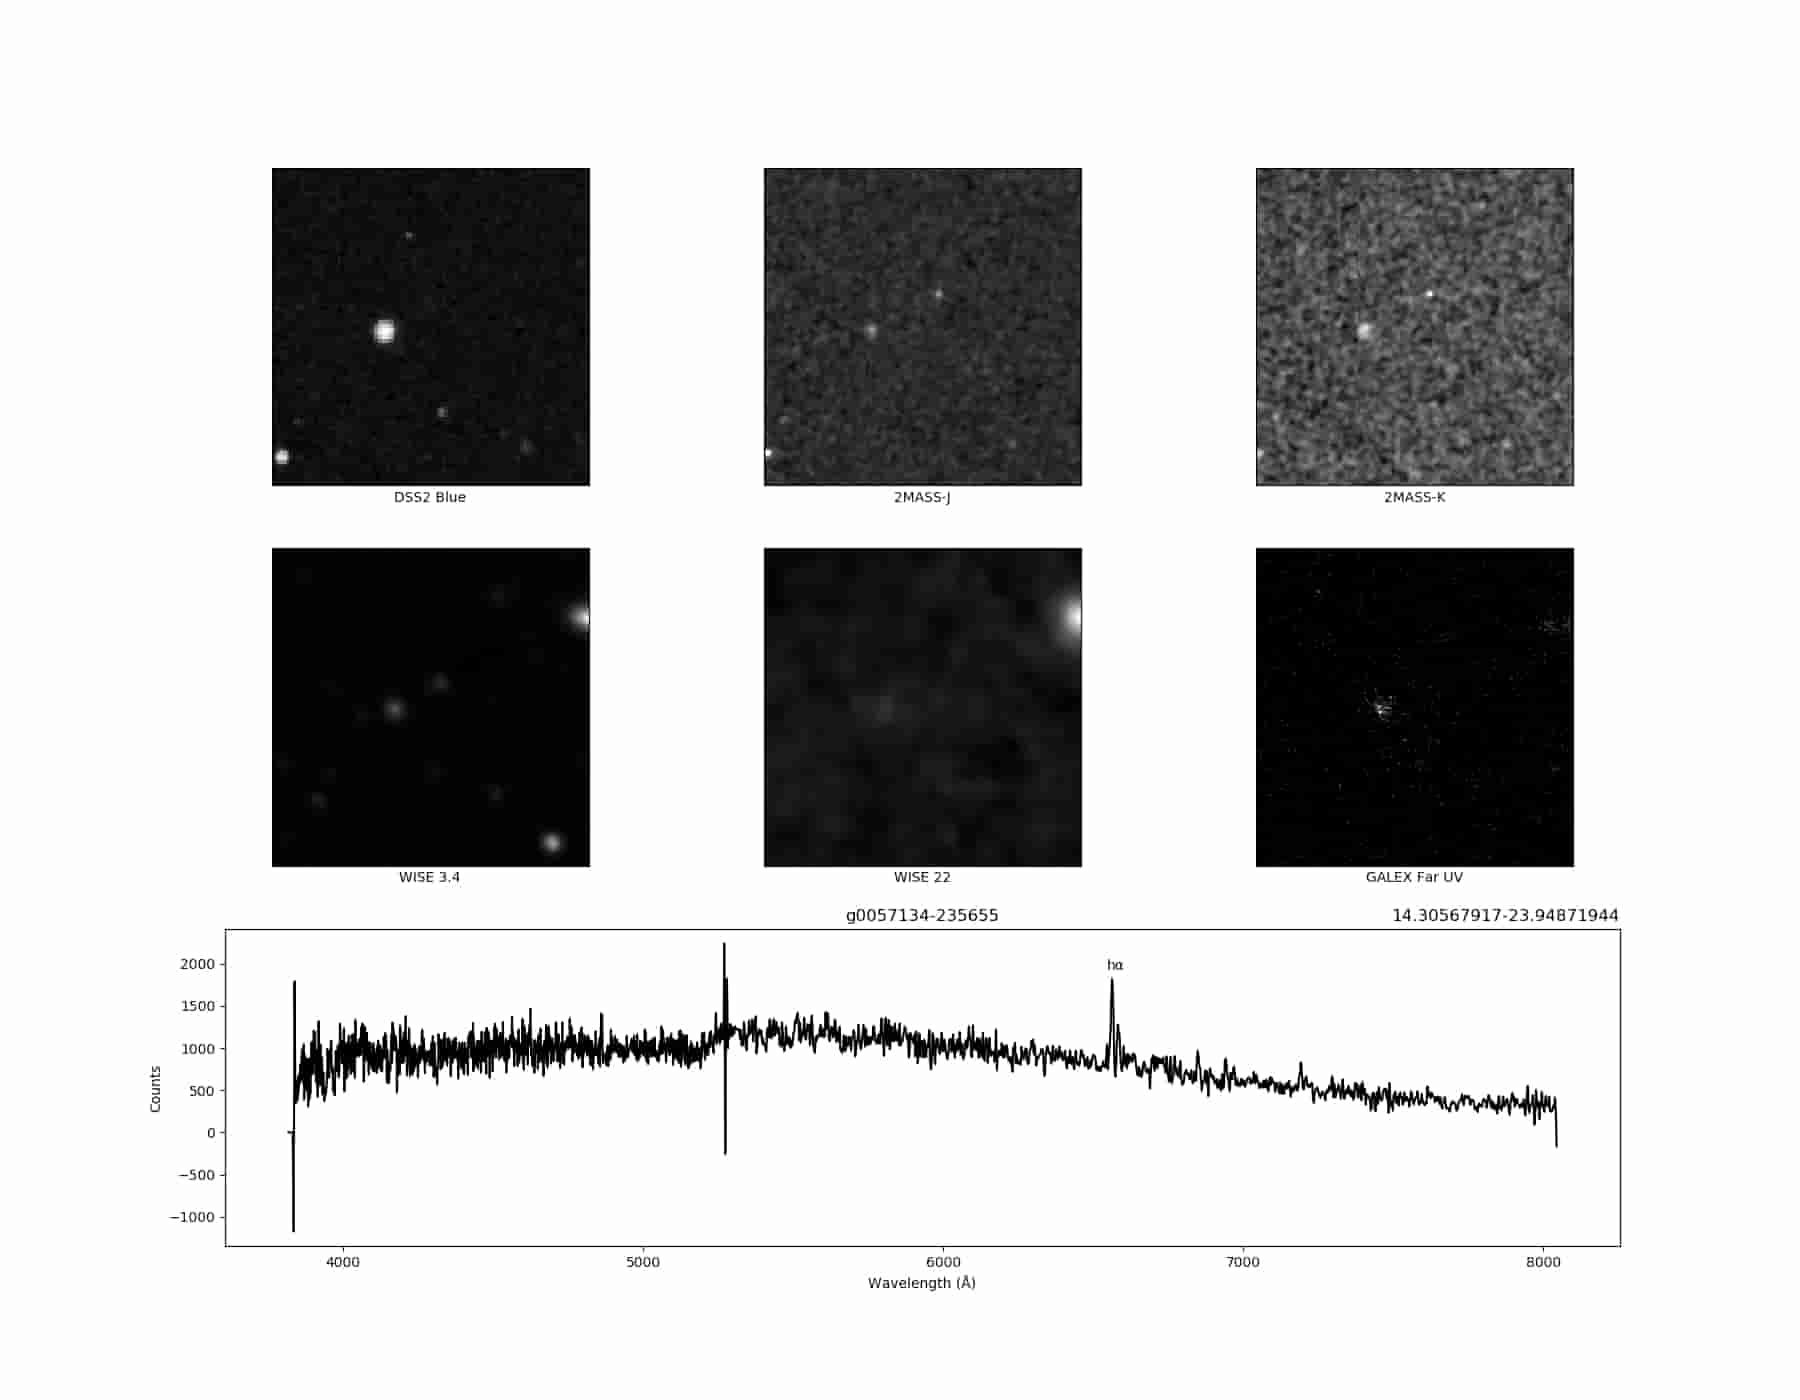
\includegraphics[scale = 0.10]{figuras/a4.jpg}
        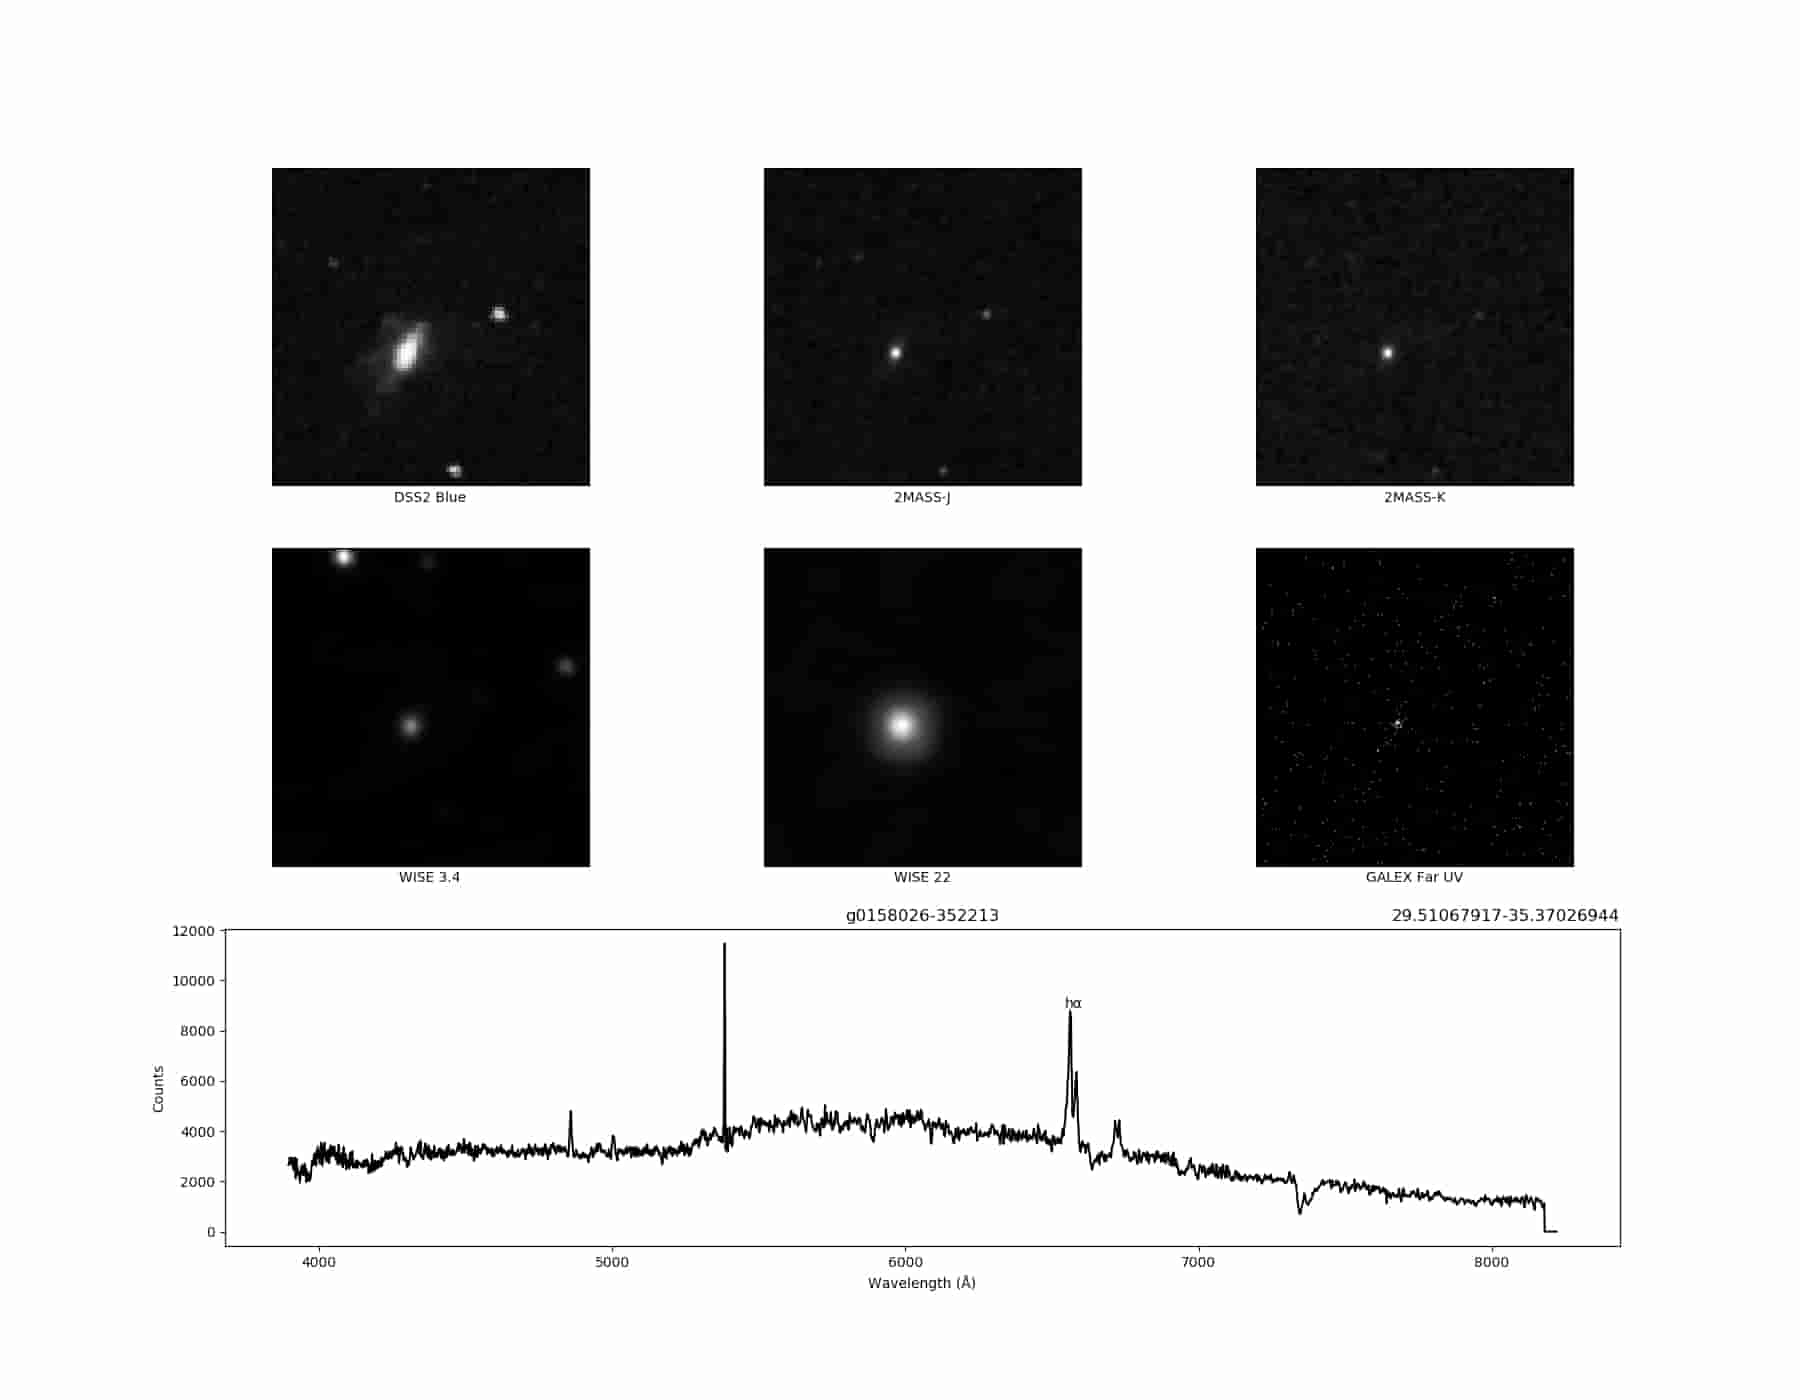
\includegraphics[scale = 0.10]{figuras/a5.jpg}
        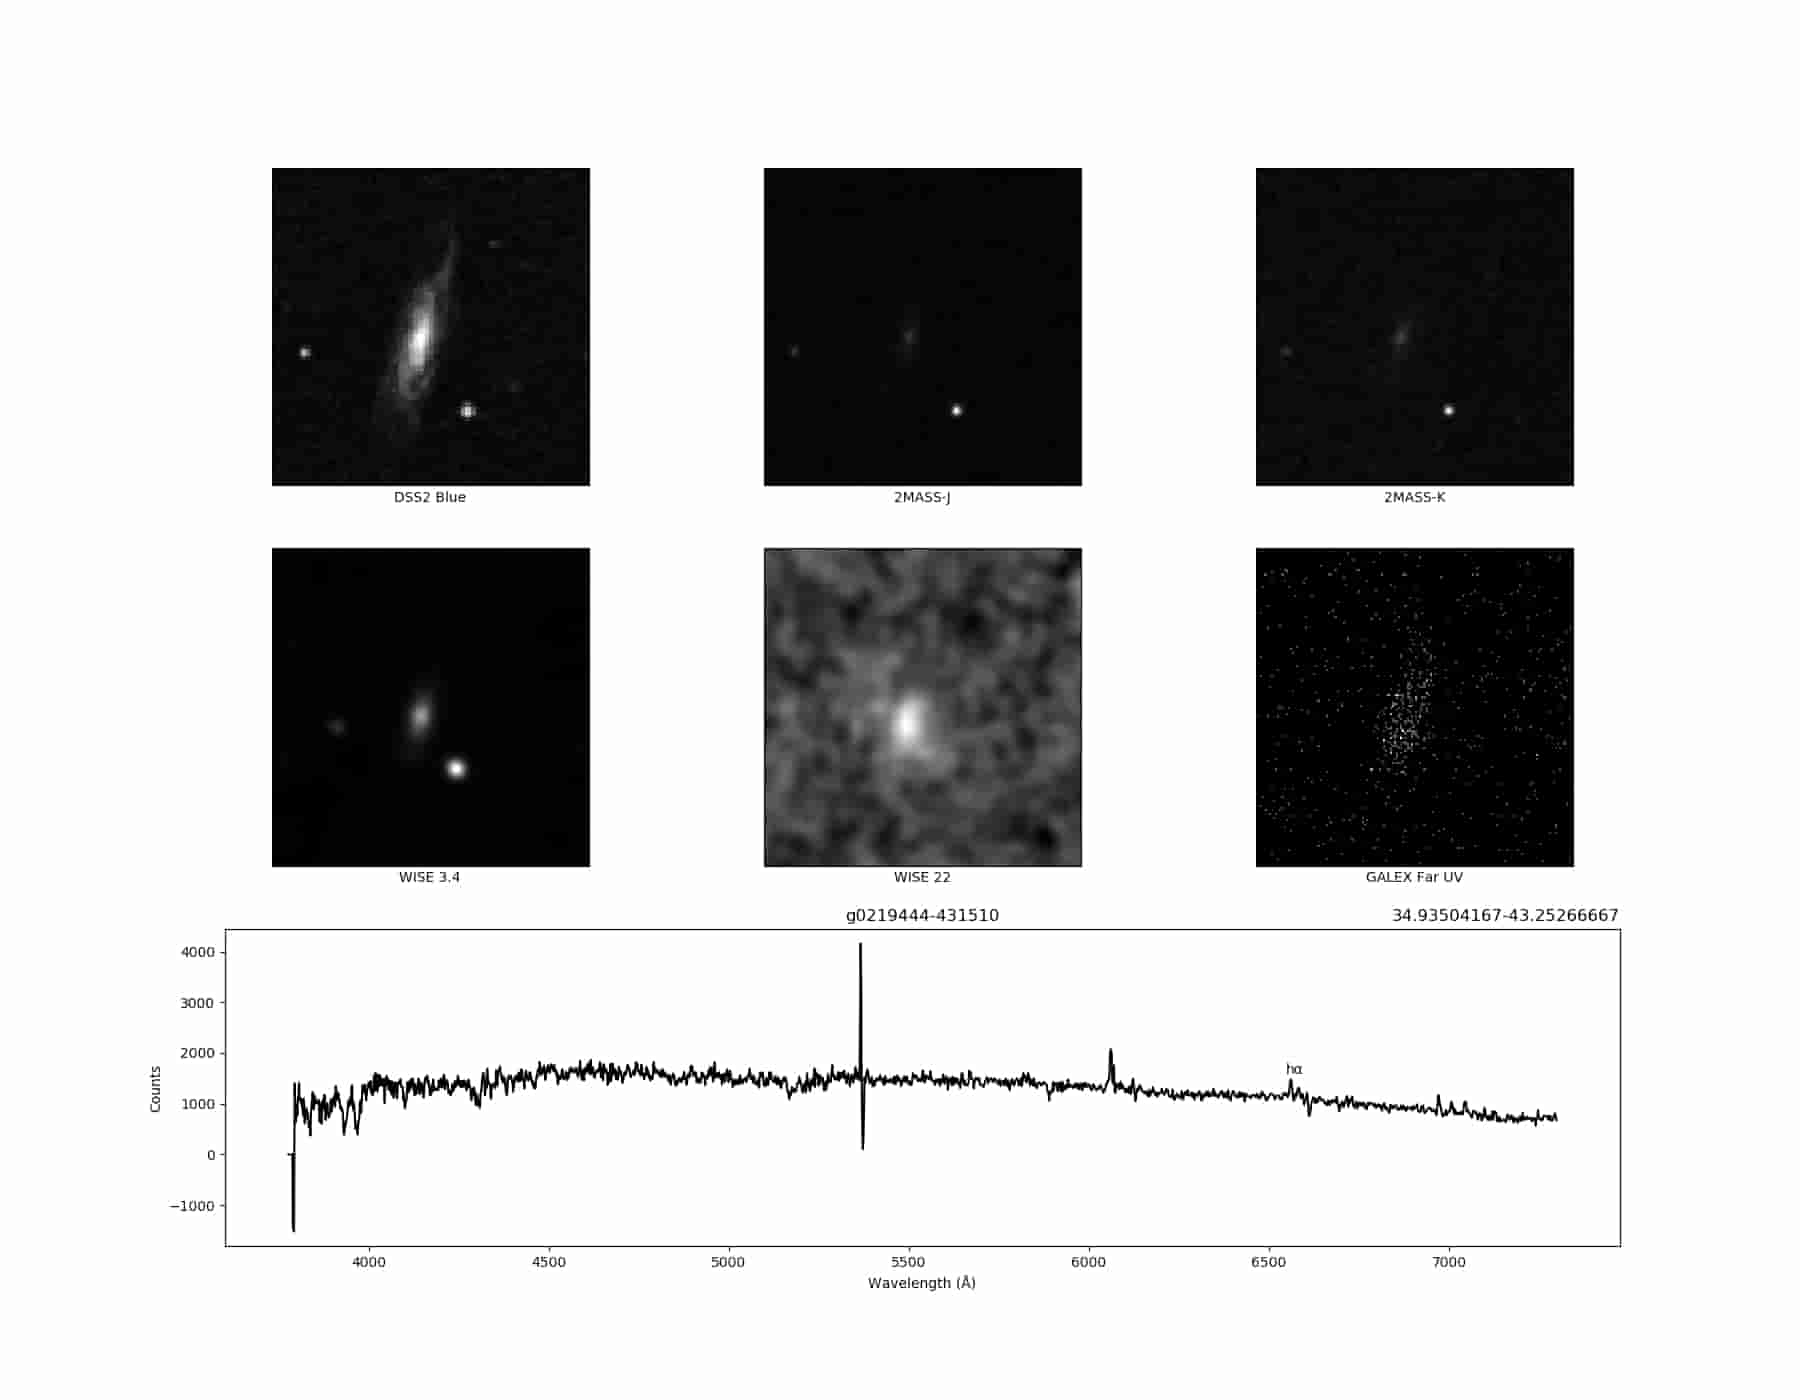
\includegraphics[scale = 0.10]{figuras/a6.jpg}
        %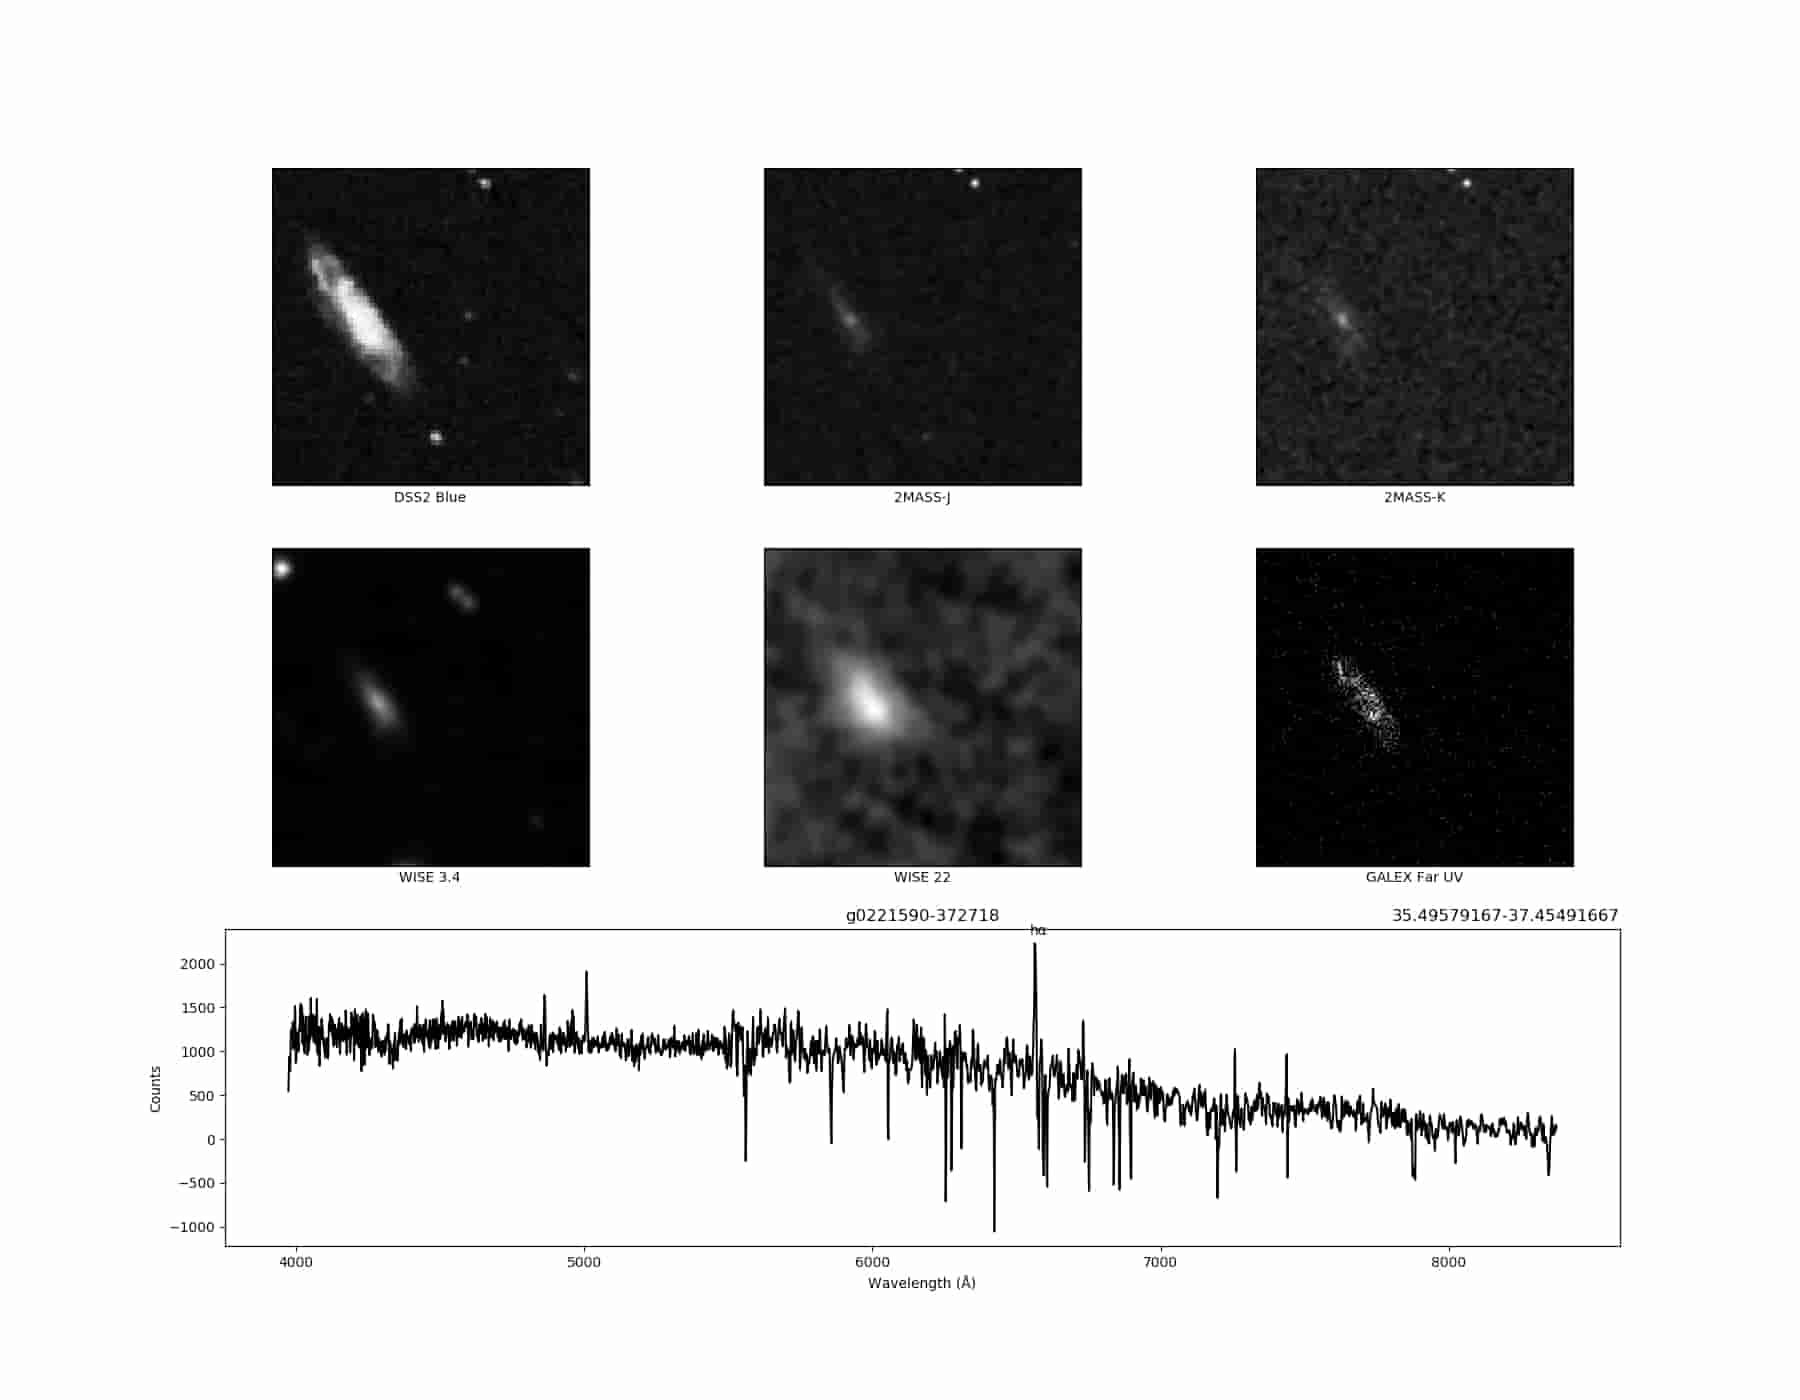
\includegraphics[scale = 0.08]{figuras/a7.jpg}
        %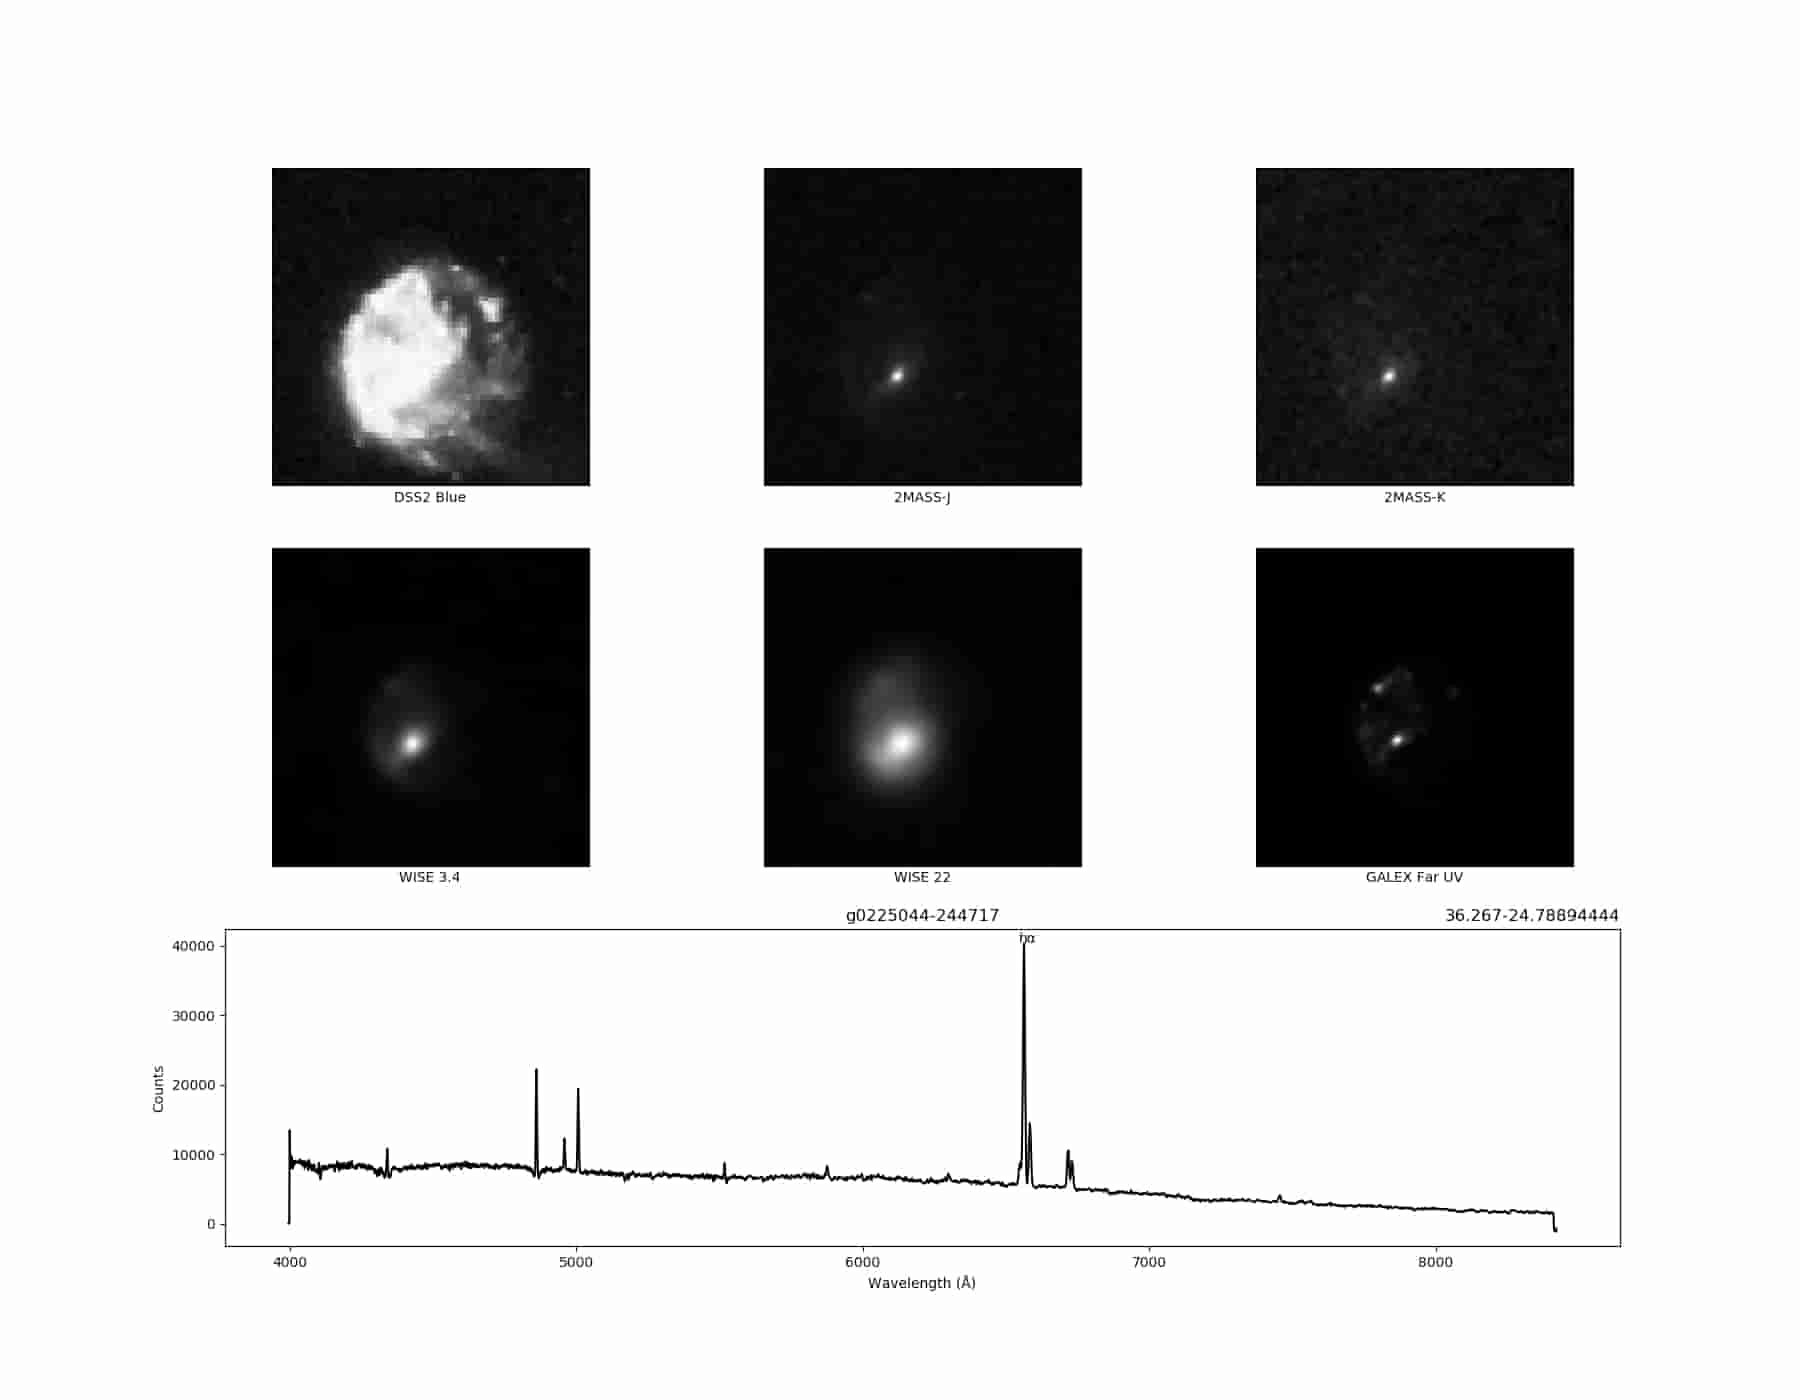
\includegraphics[scale = 0.08]{figuras/a8.jpg}
        %\caption{}
        \label{fig:my_label}
    \end{center}
\end{figure}

\chapter{Sínteses Espectrais do Starlight.}
\begin{figure}[ht!]
    \begin{center}
        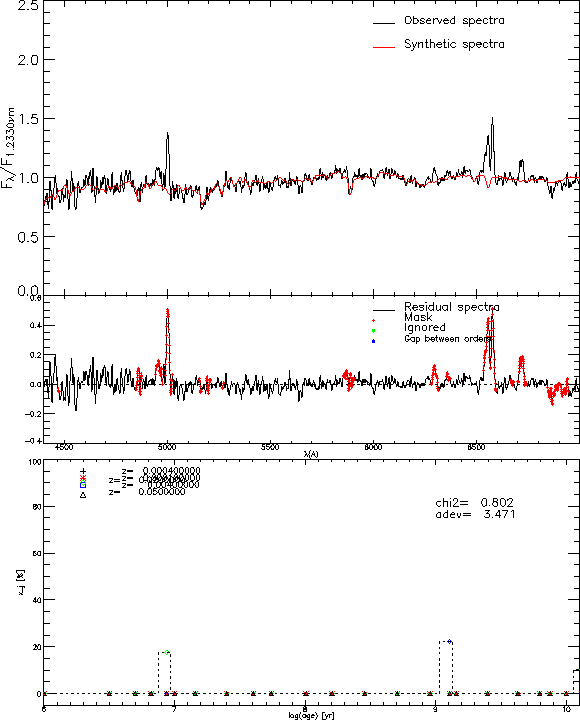
\includegraphics[scale = 0.35]{figuras/sp1.jpg}
        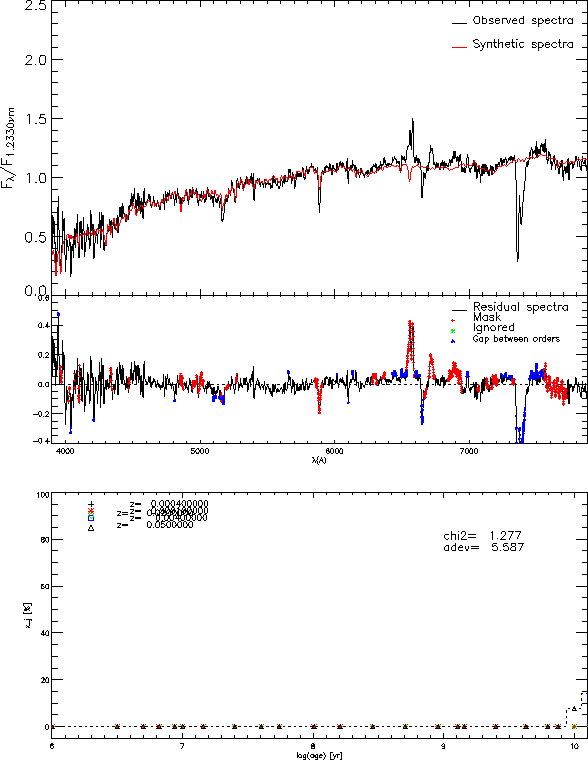
\includegraphics[scale = 0.35]{figuras/sp2.jpg}
        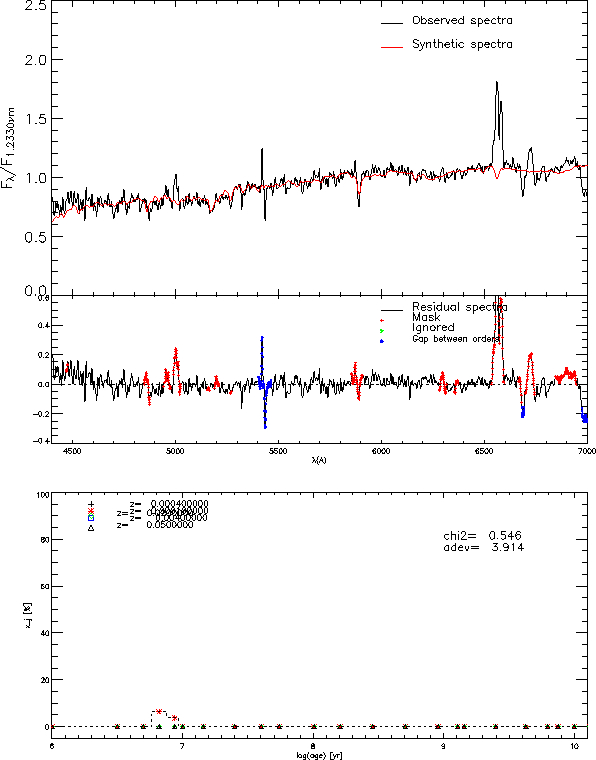
\includegraphics[scale = 0.35]{figuras/sp3.jpg}
        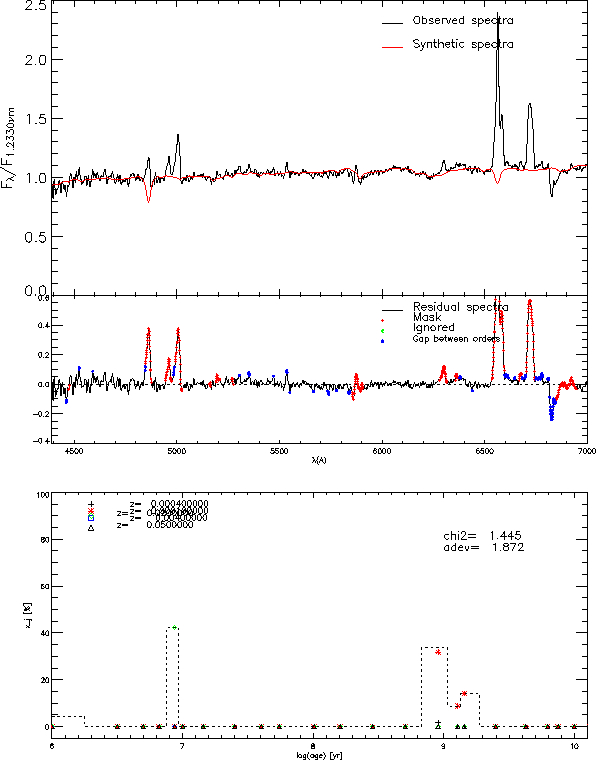
\includegraphics[scale = 0.35]{figuras/sp4.jpg}
        %\caption{}
        \label{fig:my_label}
    \end{center}
\end{figure}